\chapter{Preliminaries}
    \label{chapter:prelim}


    \section{Introduction and overview}
    

    Chapter (\ref{chapter:deformation}) starts with a review of deformation quantisation. We make the observation that what is termed a generator for a cyclic DQ module, or a \emph{wavefunction} in other literature, for example in \cite{ks_airy}, should be viewed from a sheaf theoretic perspective, as modules over a deformed sheaf of algebras. We also reprove an obstruction result for the existence of quantisation with greater clarity. This chapter is reproduced mostly from our own paper \cite{swaddledef}.
    
    Chapter (\ref{chapter:tate}) is a description of the topology required by Kontsevich and Soibelman to define Airy structures in infinite dimensions. In particular we describe the Tate space of differentials. Apart from an attempt at a clear exposition, we also incorporate details from our joint paper \cite{chaimanowong2020airy} proving some geometrical details. Chapter (\ref{chapter:infalg}) is an algebraic analog for the coordinate rings on Tate spaces. 
    
    Chapter (\ref{chapter:airy}) gives the definition of an Airy structure. Airy structures were originally defined by Kontsevich and Soibelman,  \cite{ks_airy}. Our contribution is an attempt at describing them from a more algebraic geometric perspective, and a graphical algorithm to compute terms in some resulting power series.
    
    Chapter (\ref{chapter:symplecticreduction}) explains a process known as symplectic reduction. In particular, we investigate the symplectic reduction of wavefunctions, which are defined in chapter (\ref{chapter:deformation}).
    
    Chapter (\ref{chapter:Atensor}) is based on our paper with Paul Norbury, Mehdki Tavakol and Wee Chaimanowong \cite{chaimanowong2020airy}. We mostly reproduce the contents of the paper, but it is appropriate here as it represents a coalescence of the previous chapters into an interesting result. 
    
    Previous work, \cite{chaimanowong2020airy, abcd, higherairy, eynard_orantin} studied various additional aspects of Airy structures. \cite{chaimanowong2020airy} was primarily concerned with aspects of symplectic reduction, while \cite{abcd} studies classifications of Airy structures. Following ideas from Kontsevich and Soibelman, the overall goal of this thesis is to fill in a missing link, and relate aspects of \emph{Airy structures} and \emph{topological recursion} using \emph{deformation quantisation}. The deformation quantisation aspect was not present in \cite{chaimanowong2020airy} and \cite{abcd}, and leads to interesting insight into the objects known as wavefunctions.

    
    
    \section{Eynard-Orantin Topological recursion}


    \emph{\hyperref[defn:tr]{Topological recursion}}, by Eynard and Orantin \cite{eynard_orantin}, is a recursive algorithm in two non-negative integers \((g,n)\), which produces a collection of symmetric, poly-differentials, \(\omega_{g,n}\). Many interesting invariants arising from problems in enumerative geometry and string theory can be computed by topological recursion, via different choices of the initial data given by \(\omega_{0,3}\) and \(\omega_{1,1}\). Topological recursion was first studied in the context of free energies of matrix models \cite{CEyHer}. The initial data can be encoded in an object called a \emph{\hyperref[defn:spectral_curve]{spectral curve}}.
    
    We give a slightly different definition of spectral curve
    to bridge the difference between the definition in \cite{eynard_orantin} and \cite{ks_airy}. Let \((X,\mathcal{O}_X) \) be a scheme over a field \( \mathbf{k}\) of characteristic zero, usually \( \mathbb{C}\).
    \begin{defn}[Weil divisor] A \emph{divisor} \(D\) on \(X\) is a formal \(\mathbb{Z}\)-linear combination 
    \[ D = \sum_j k_j Z_j,\]
    where \(Z_j\) is a codimension 1 subscheme, \(k_j \in \mathbb{Z}\).
    \end{defn}
    %If \(X\) is a Riemann surface, codimension 1 submanifolds are points.
    %Recall the space of K\"ahler (holomorphic) differentials is denoted \( \Omega_{\Sigma/\mathbb{C}}\). 
    %The de-Rahm complex is \( \Omega^n_{\Sigma/\mathbb{C}} = \bigwedge^n \Omega_{\Sigma/\mathbb{C}}\).
    
    %\begin{defn}[Symmetric bi-differential]
    %\end{defn}
    Now let \( (X,\mathcal{O}_X)\) be a complex algebraic surface. For any Weil divisor \(D\) there is an associated sub-sheaf \( \mathcal{O}_X(D)\), of the sheaf  of rational functions \(\mathcal{K}_X\) on \(X\). \( D\) is called \emph{Cartier} if \( \mathcal{O}_X(D)\) is an invertible sheaf. Let \( \mathcal{M}_X\) be the sheaf of meromorphic functions.
    

    
    \begin{defn}[Spectral curve]
    \label{defn:spectral_curve} 
    The tuple \( ( \Sigma, x,y,B)\) is called a \emph{spectral curve} where:
    
    
    \begin{itemize} 
    \item \( \Sigma \) is a Riemann surface.

    \item \(D_\Sigma \) is a Cartier divisor.
    
    \item \(x \in  \mathcal{O}_\Sigma(D_\Sigma)\) is a meromorphic function, such that \(dx \in  \Omega_{\Sigma}^1 (D_\Sigma)\) is algebraic, and zeros of \(dx\) are simple. Note \(D_\Sigma\) allows for arbitrary order poles at points.
    
    \item  \(y \in  \mathcal{M}_\Sigma\) is a meromorphic function regular at \(D_\Sigma \).

    \item  \( B \in H^0( \Sigma \times \Sigma, (\Omega_\Sigma^1 \boxtimes \Omega_\Sigma^1)(2 \triangle)) \) is a global symmetric bi-differential, \( \triangle = \mathrm{diag}(\Sigma \times \Sigma) \).
    \end{itemize}
    
    
    \end{defn}
    Later this data will be specified by a  \emph{foliation} on a symplectic surface \(X\). \( \Sigma\) becomes a curve in \(X\), \( \Sigma \rightarrow X\). The foliation defines a divisor \(D\), and then \(D_\Sigma = D \cap \Sigma\). 
    
    \begin{rem}
    \(x\) and \(y\) give a local and possibly global embedding of \(\Sigma \) into \( \mathbb{C}^2\).
    In the latter cases, this can be considered a subvariety generated by an ideal \( \langle P(x,y)\rangle\), in \( \mathbf{k}[x,y]\), where \(P(x,y)\) is a polynomial.
    \end{rem}
    
    
    
    %gives local (possibly global) embedding into \( \mathbb{C}^2\),
    
    % x,y local embedding in C^2
    %eynard oratin start with curve in C^2
    
    %Define the divisor \(R\) as the formal combination of order and zeroes of \(dx\).
    
    Consider a spectral curve \( (\Sigma,x,y,B)\).
    Define the divisor \(R\) as the simple zeros of \(dx\): 
    \[ R = \{ \alpha : d x(\alpha) = 0 \} \]
    Consider \( \alpha \in  R\), and \( U_{\alpha} \subset \Sigma\) be an open neighbourhood around \(\alpha\).
    %\begin{defn}[Galois involution] A \emph{Galois involution} is a locally defined map \(\sigma : U \rightarrow U\), such that \( x = x \cdot \sigma \).
    %\end{defn}
    %Recall in complex analysis, the residue of a complex function \(f\) along a closed curve \( \gamma\) is defined as \[\Res(f,\gamma) = \frac{1}{2 \pi i} \oint_\gamma f d z. \] 
    %\begin{defn}[Residue] The \emph{residue} is a linear functional, pairing a complex differential with a cycle:
    %\[ \Res : H^1(\Sigma,\mathbf{k}) \rightarrow H_1(\Sigma,\mathbb{Z}) \rightarrow \mathbf{k}.\]
    %\end{defn} 
    %The residue defines a symplectic form on the space of meromorphic differentials.
    %\begin{lem}[Symplectic form from residue]
    %\[ \omega(\psi,\eta) = \sum_{\alpha \in D_\Sigma } %\mathrm{Res}(f \eta, \alpha), \]
    %where locally \( d f = \psi\).
    %\end{lem}
    \begin{defn}[Local Galois involution]
    A \emph{local Galois involution} is a map defined locally around \(\alpha \in R\), and must satisfy \( x( \sigma_{\alpha}(p)) = x(p)\) for \( p \in U_{\alpha}\), \( \sigma_{\alpha}(\alpha) = \alpha \), \( \sigma_{\alpha}(p) \neq p\), for \(p \neq \alpha \in U_{\alpha}\).
    \end{defn}
    This definition uniquely determines \( \sigma_{\alpha}\).
    
    \begin{defn}[Recursion kernel]
    The \emph{recursion kernel} is a locally defined function \( K : U_{\alpha} \times U_{\alpha} \rightarrow \mathbb{C}\).
    \[ K(p_1, p)  = -\frac{1}{2} \ddfrac{\int_{\sigma_{\alpha}(p)}^{p} dw \, B(p_1,w)}{(y(p) - y(\sigma(p))) \, dx(p)}. \]
    \end{defn}
    Note the cancellation of the differentials.
    
    
    From the initial data of a spectral curve \((\Sigma, x,y,B)\) define two meromorphic differentials, \( \omega_{0,1}(p_1) = y(p_1) dx(p_1)\) and \( \omega_{0,2}(p_1, p_2) = B(p_1,p_2)\), and \(p\) is a local coordinate on \( \Sigma\).
    
    \begin{defn}[Topological recursion]\label{defn:tr} \emph{Topological recursion} is the collection of tensor products of meromorphic differentials \( \omega_{g,n} \in  H^0((\Sigma \setminus D_\Sigma)^n,(\Omega^1_\Sigma)^{\boxtimes n})\), which we call polydifferentials, defined by the quadratic recursive formula as follows:
    \begin{align*} 
    \omega_{g,n}(p_1, \dots p_n) =& \sum_{\alpha \in R } \Res_{z = \alpha}  K(p_1, p)     \Big( \omega_{g-1, n+1} (p, \sigma_\alpha(p), p_2, \dots, p_n) \\
        &+ \sum^{'}_{\substack{g_1 + g_2 = g \\ I_1 \sqcup \, I_2 = \{p_2\dots,p_n\} }} \omega_{g_1, \# I_1+1}(p,I_1) \, \omega_{g_2, \#I_2  +1}(\sigma_{\alpha}(p), I_2) \Big),
    \end{align*}
    where the \( \sum^{'}\) denotes excluding \((g,n)=(0,1)\) terms, \( \sigma_{\alpha}\) is a local Galois involution around \( \alpha\), and \( \#\) denotes size of a partition.
    \end{defn}
    The polydifferentials \(\omega_{g,n}(p_1,..., p_n)\) are tensor products of meromorphic differentials, and are symmetric in \(p_i\) \cite{eynard_orantin}. Furthermore they have zero residue poles at \(p_i=\alpha\) for any zero \( \alpha \in R\) of \(dx\), and are holomorphic outside \(R\). 

    There is a natural choice of symmetric bi-differential \(B\) called the \emph{Bergman kernel} on \( \Sigma\). First recall that associated to \( \Sigma\) is a choice of basis of homology:
    \begin{defn}[Torelli marked basis]
    A \emph{Torelli marked basis} \cite{bertola}, is a choice of \(2g\) cycles of homology \[  \{a_1, \dots a_g, b_1, \dots b_g\} \subset H_1(\Sigma, \mathbb{Z}).\]
    \end{defn}

    %look in paper and fix
    
    Now let \( \Sigma\) have a Torelli marked basis, with a choice of \(a\)-cycles, \( \{a_i\}_{i=1,...,g}\subset\Sigma\).
    \begin{defn}[Bergman kernel]
    The \emph{Bergman kernel} \(B(p,w)\), is a canonical, normalised, symmetric \(B(w,p)=B(p,w)\), meromorphic, bi-differential on \( \Sigma \times \Sigma\).  It is normalised by 
    \[ \int_{p \in a_i}B(p,w)=0 \quad i=1,\dots,g. \]
    In terms of a local coordinate \(u\) on \( \Sigma\), it is given by
    \[ B(p,w)=\frac{du(p)du(w)}{(u(p)-u(w))^2}+\mathrm{holo}(u(p),u(w)) \]
    where \( \mathrm{holo}\) means some holomorphic function.
    \end{defn}
    With the choice of Bergman kernel in topological recursion, the \( \omega_{g,n}\) inherit from \(B(z,w)\), the property that 
    \[ \int_{p_1 \in a_k}\omega_{g,n}(p_1,\cdots,p_n) = 0.\]
    
    
    Topological recursion depends only on a neighbourhood of the zeros of \(dx\), hence \(x\), \(y\) and \(B\) need only be defined locally in these neighbourhoods:
    %check paper
    \begin{defn}[Local spectral curve]
    \label{defn:localspectral}
    When \(x\), \(y\) and \(B\) are only defined locally in a neighbourhoods of zeros of \(dx\), or a point in \(R\), \((\Sigma,x,y,B)\) is  said to be a \emph{local spectral curve}.
    \end{defn}
    In chapter (\ref{chapter:Atensor}), \(x\) and \(y\) will be coordinates around points \(\alpha\) in a divisor \(R\), \( \alpha \in R\). In this situation we will use the notation \( x = u_{\alpha}\), \(y= v_{\alpha}\).

    
    Topological recursion can be represented graphically by figure (\ref{fig:tr}).
    \begin{figure}[!htb]
        \centering 
        \tikzset{every picture/.style={line width=0.75pt}} %set default line width to 0.75pt        

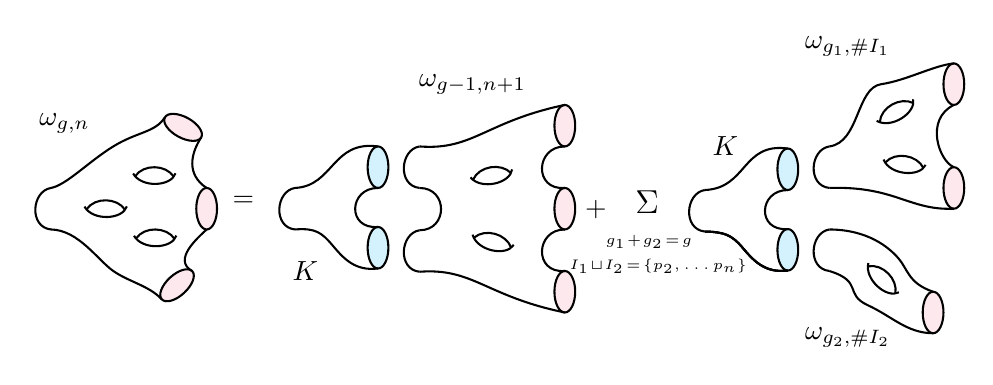
\begin{tikzpicture}[x=0.75pt,y=0.75pt,yscale=-1,xscale=1]
%uncomment if require: \path (0,190); %set diagram left start at 0, and has height of 190

%Shape: Ellipse [id:dp47766951388601575] 
\draw  [fill={rgb, 255:red, 85; green, 205; blue, 252 }  ,fill opacity=0.25 ] (162.56,69.5) .. controls (162.56,63.98) and (164.8,59.5) .. (167.56,59.5) .. controls (170.32,59.5) and (172.56,63.98) .. (172.56,69.5) .. controls (172.56,75.02) and (170.32,79.5) .. (167.56,79.5) .. controls (164.8,79.5) and (162.56,75.02) .. (162.56,69.5) -- cycle ;
%Shape: Ellipse [id:dp2213117305497102] 
\draw  [fill={rgb, 255:red, 85; green, 205; blue, 252 }  ,fill opacity=0.25 ] (162.56,108.3) .. controls (162.56,102.78) and (164.8,98.3) .. (167.56,98.3) .. controls (170.32,98.3) and (172.56,102.78) .. (172.56,108.3) .. controls (172.56,113.83) and (170.32,118.3) .. (167.56,118.3) .. controls (164.8,118.3) and (162.56,113.83) .. (162.56,108.3) -- cycle ;
%Curve Lines [id:da6254818543814082] 
\draw    (127.56,79.5) .. controls (146.2,78.6) and (145.39,56.5) .. (167.56,59.5) ;
%Curve Lines [id:da26678157319223816] 
\draw    (127.56,99.5) .. controls (137.49,98.7) and (140.48,101.08) .. (145.58,107.07) .. controls (150.67,113.06) and (156.21,119.75) .. (167.56,118.3) ;
%Shape: Ellipse [id:dp13037643339418226] 
\draw  [fill={rgb, 255:red, 85; green, 205; blue, 252 }  ,fill opacity=0.25 ] (360,70.5) .. controls (360,64.98) and (362.24,60.5) .. (365,60.5) .. controls (367.76,60.5) and (370,64.98) .. (370,70.5) .. controls (370,76.02) and (367.76,80.5) .. (365,80.5) .. controls (362.24,80.5) and (360,76.02) .. (360,70.5) -- cycle ;
%Shape: Ellipse [id:dp17263407292053756] 
\draw  [fill={rgb, 255:red, 85; green, 205; blue, 252 }  ,fill opacity=0.25 ] (360,109.3) .. controls (360,103.78) and (362.24,99.3) .. (365,99.3) .. controls (367.76,99.3) and (370,103.78) .. (370,109.3) .. controls (370,114.82) and (367.76,119.3) .. (365,119.3) .. controls (362.24,119.3) and (360,114.82) .. (360,109.3) -- cycle ;
%Curve Lines [id:da07654552783686674] 
\draw    (325,80.5) .. controls (345.53,79.6) and (342.83,57.5) .. (365,60.5) ;
%Curve Lines [id:da9658431109856747] 
\draw    (325,100.5) .. controls (334.27,100.7) and (337.92,102.08) .. (343.02,108.07) .. controls (348.11,114.06) and (353.65,120.74) .. (365,119.3) ;
%Curve Lines [id:da5347071930943992] 
\draw    (365,80.5) .. controls (350.83,80.5) and (349.83,100.5) .. (365,99.3) ;
%Shape: Ellipse [id:dp3047856800313534] 
\draw  [fill={rgb, 255:red, 247; green, 168; blue, 184 }  ,fill opacity=0.25 ] (440,29.5) .. controls (440,23.98) and (442.24,19.5) .. (445,19.5) .. controls (447.76,19.5) and (450,23.98) .. (450,29.5) .. controls (450,35.02) and (447.76,39.5) .. (445,39.5) .. controls (442.24,39.5) and (440,35.02) .. (440,29.5) -- cycle ;
%Shape: Ellipse [id:dp604261263939661] 
\draw  [fill={rgb, 255:red, 247; green, 168; blue, 184 }  ,fill opacity=0.25 ] (440,79.5) .. controls (440,73.98) and (442.24,69.5) .. (445,69.5) .. controls (447.76,69.5) and (450,73.98) .. (450,79.5) .. controls (450,85.02) and (447.76,89.5) .. (445,89.5) .. controls (442.24,89.5) and (440,85.02) .. (440,79.5) -- cycle ;
%Shape: Ellipse [id:dp011621115124847092] 
\draw  [fill={rgb, 255:red, 247; green, 168; blue, 184 }  ,fill opacity=0.25 ] (430,139.5) .. controls (430,133.98) and (432.24,129.5) .. (435,129.5) .. controls (437.76,129.5) and (440,133.98) .. (440,139.5) .. controls (440,145.02) and (437.76,149.5) .. (435,149.5) .. controls (432.24,149.5) and (430,145.02) .. (430,139.5) -- cycle ;
%Curve Lines [id:da570536589787372] 
\draw    (385,59.5) .. controls (399.53,57.6) and (397.98,31.23) .. (410,29.5) .. controls (422.02,27.77) and (435.36,20.43) .. (445,19.5) ;
%Curve Lines [id:da47026968306688344] 
\draw    (385,79.5) .. controls (416.83,78.5) and (423.36,90.43) .. (445,89.5) ;
%Curve Lines [id:da10402241670297141] 
\draw    (445,39.5) .. controls (430.83,46.5) and (437.83,66.5) .. (445,69.5) ;
%Curve Lines [id:da7257812222165501] 
\draw    (411.92,67.27) .. controls (416.75,61.8) and (427.35,63.59) .. (430.34,69.91) ;
%Curve Lines [id:da1333862640100011] 
\draw    (411.13,65.82) .. controls (414.17,73.32) and (428.46,74.53) .. (431.39,68.4) ;

%Curve Lines [id:da9669557373363992] 
\draw    (409.32,47.82) .. controls (409.79,40.54) and (419.25,35.45) .. (425.49,38.61) ;
%Curve Lines [id:da3422827424389957] 
\draw    (407.81,47.17) .. controls (414.82,51.22) and (426.83,43.4) .. (425.39,36.77) ;

%Curve Lines [id:da9799334827307091] 
\draw    (385,119.5) .. controls (401.6,124.7) and (391.85,130.63) .. (403.6,136.03) .. controls (415.35,141.43) and (422.35,149.43) .. (435,149.5) ;
%Curve Lines [id:da9139019865430383] 
\draw    (403.59,117.28) .. controls (410.73,115.78) and (418.17,123.53) .. (416.8,130.39) ;
%Curve Lines [id:da4926725298466649] 
\draw    (403.81,115.66) .. controls (401.79,123.49) and (412.53,132.97) .. (418.54,129.8) ;

%Curve Lines [id:da8231578381022252] 
\draw    (385,99.5) .. controls (403.53,99.6) and (413.6,108.03) .. (418.27,113.37) .. controls (422.93,118.7) and (422.93,125.37) .. (435,129.5) ;
%Curve Lines [id:da41952521800040865] 
\draw    (325,80.5) .. controls (315.6,82.03) and (314.27,99.37) .. (325,100.5) ;
%Curve Lines [id:da022423481574913584] 
\draw    (385,59.5) .. controls (375.6,61.03) and (374.27,78.37) .. (385,79.5) ;
%Curve Lines [id:da9251927665164891] 
\draw    (385,99.5) .. controls (375.6,101.03) and (374.27,118.37) .. (385,119.5) ;
%Curve Lines [id:da23000894520127613] 
\draw    (325,100.5) .. controls (334.27,100.7) and (337.92,102.08) .. (343.02,108.07) .. controls (348.11,114.06) and (353.65,120.74) .. (365,119.3) ;
%Curve Lines [id:da10195049737374684] 
\draw    (167.56,79.5) .. controls (153.39,79.5) and (152.39,99.5) .. (167.56,98.3) ;
%Curve Lines [id:da5107062925199526] 
\draw    (187.56,79.5) .. controls (201.39,79.5) and (201.39,99.88) .. (187.56,99.88) ;
%Shape: Ellipse [id:dp3889460224785426] 
\draw  [fill={rgb, 255:red, 247; green, 168; blue, 184 }  ,fill opacity=0.26 ] (252.56,49.5) .. controls (252.56,43.98) and (254.8,39.5) .. (257.56,39.5) .. controls (260.32,39.5) and (262.56,43.98) .. (262.56,49.5) .. controls (262.56,55.02) and (260.32,59.5) .. (257.56,59.5) .. controls (254.8,59.5) and (252.56,55.02) .. (252.56,49.5) -- cycle ;
%Shape: Ellipse [id:dp9770499883484128] 
\draw  [fill={rgb, 255:red, 247; green, 168; blue, 184 }  ,fill opacity=0.25 ] (252.56,89.5) .. controls (252.56,83.98) and (254.8,79.5) .. (257.56,79.5) .. controls (260.32,79.5) and (262.56,83.98) .. (262.56,89.5) .. controls (262.56,95.02) and (260.32,99.5) .. (257.56,99.5) .. controls (254.8,99.5) and (252.56,95.02) .. (252.56,89.5) -- cycle ;
%Shape: Ellipse [id:dp4597094401087267] 
\draw  [fill={rgb, 255:red, 247; green, 168; blue, 184 }  ,fill opacity=0.25 ] (252.56,129.5) .. controls (252.56,123.98) and (254.8,119.5) .. (257.56,119.5) .. controls (260.32,119.5) and (262.56,123.98) .. (262.56,129.5) .. controls (262.56,135.02) and (260.32,139.5) .. (257.56,139.5) .. controls (254.8,139.5) and (252.56,135.02) .. (252.56,129.5) -- cycle ;
%Shape: Boxed Bezier Curve [id:dp4201913915112617] 
\draw    (187.56,59.5) .. controls (213.39,61.5) and (219.39,47.5) .. (257.56,39.5) ;
%Curve Lines [id:da17496795078002492] 
\draw    (257.56,59.5) .. controls (243.39,59.5) and (242.39,80.7) .. (257.56,79.5) ;
%Straight Lines [id:da8933167588243608] 
\draw  [dash pattern={on 4.5pt off 4.5pt}]  (222.56,89.5) ;
%Shape: Boxed Bezier Curve [id:dp20175324397284145] 
\draw    (187.56,119.88) .. controls (213.39,117.92) and (219.39,131.65) .. (257.56,139.5) ;
%Curve Lines [id:da7870873777983136] 
\draw    (257.56,99.5) .. controls (243.39,99.5) and (242.39,120.7) .. (257.56,119.5) ;
%Curve Lines [id:da8945713210334673] 
\draw    (325,100.5) .. controls (334.27,100.7) and (337.92,102.08) .. (343.02,108.07) .. controls (348.11,114.06) and (353.65,120.74) .. (365,119.3) ;
%Curve Lines [id:da6694044469732641] 
\draw    (213.33,75.57) .. controls (216.22,68.88) and (226.84,67.26) .. (231.66,72.34) ;
%Curve Lines [id:da5731533719506826] 
\draw    (212.13,74.45) .. controls (217.37,80.62) and (231.31,77.31) .. (232.18,70.57) ;

%Curve Lines [id:da02679938946556648] 
\draw    (213.73,103.52) .. controls (219.18,98.67) and (229.49,101.69) .. (231.71,108.32) ;
%Curve Lines [id:da8638414158098124] 
\draw    (213.12,102) .. controls (215.26,109.8) and (229.3,112.68) .. (232.93,106.94) ;

%Curve Lines [id:da5955732991885125] 
\draw    (187.56,59.5) .. controls (178.16,61.03) and (176.82,78.37) .. (187.56,79.5) ;
%Curve Lines [id:da21844641699333922] 
\draw    (187.56,99.88) .. controls (178.16,101.42) and (176.82,118.75) .. (187.56,119.88) ;
%Curve Lines [id:da22082602480849645] 
\draw    (127.56,79.5) .. controls (118.16,81.03) and (116.82,98.37) .. (127.56,99.5) ;
%Shape: Ellipse [id:dp047839199679800104] 
\draw  [fill={rgb, 255:red, 247; green, 168; blue, 184 }  ,fill opacity=0.26 ] (76.04,45.92) .. controls (80.88,48.58) and (83.73,52.69) .. (82.4,55.12) .. controls (81.08,57.54) and (76.07,57.35) .. (71.23,54.69) .. controls (66.39,52.04) and (63.54,47.92) .. (64.87,45.5) .. controls (66.19,43.08) and (71.19,43.27) .. (76.04,45.92) -- cycle ;
%Shape: Ellipse [id:dp8497917036559762] 
\draw  [fill={rgb, 255:red, 247; green, 168; blue, 184 }  ,fill opacity=0.26 ] (80,89.5) .. controls (80,83.98) and (82.24,79.5) .. (85,79.5) .. controls (87.76,79.5) and (90,83.98) .. (90,89.5) .. controls (90,95.02) and (87.76,99.5) .. (85,99.5) .. controls (82.24,99.5) and (80,95.02) .. (80,89.5) -- cycle ;
%Curve Lines [id:da21030774171420585] 
\draw    (27.11,89.81) .. controls (31.19,83.76) and (41.93,84.15) .. (45.72,90.03) ;
%Curve Lines [id:da2054533399102827] 
\draw    (26.14,88.48) .. controls (30.14,95.52) and (44.45,94.85) .. (46.56,88.39) ;

%Curve Lines [id:da2922985882802336] 
\draw    (50.55,73.87) .. controls (54.63,67.82) and (65.37,68.2) .. (69.16,74.08) ;
%Curve Lines [id:da7481414220068059] 
\draw    (49.58,72.54) .. controls (53.58,79.58) and (67.89,78.9) .. (70,72.45) ;

%Curve Lines [id:da19338719689530326] 
\draw    (50.97,103.87) .. controls (55.05,97.82) and (65.79,98.2) .. (69.58,104.08) ;
%Curve Lines [id:da4856907558404082] 
\draw    (50,102.54) .. controls (54,109.58) and (68.32,108.9) .. (70.42,102.45) ;

%Shape: Ellipse [id:dp5786014847995782] 
\draw  [fill={rgb, 255:red, 247; green, 168; blue, 184 }  ,fill opacity=0.26 ] (74.13,130.06) .. controls (70.07,133.81) and (65.27,135.2) .. (63.39,133.17) .. controls (61.52,131.14) and (63.29,126.46) .. (67.35,122.71) .. controls (71.4,118.97) and (76.21,117.57) .. (78.08,119.6) .. controls (79.96,121.63) and (78.19,126.31) .. (74.13,130.06) -- cycle ;
%Curve Lines [id:da5518785962687732] 
\draw    (10,79.5) .. controls (0.6,81.03) and (-0.73,98.37) .. (10,99.5) ;
%Curve Lines [id:da9074172955656375] 
\draw    (10,99.5) .. controls (23.24,99.75) and (32.51,114.27) .. (40,119.5) .. controls (47.49,124.73) and (57.39,126.65) .. (63.39,133.17) ;
%Curve Lines [id:da4486713212196154] 
\draw    (10,79.5) .. controls (17.34,78.17) and (28.21,66.73) .. (40,59.5) .. controls (51.79,52.27) and (60.13,52.87) .. (64.87,45.5) ;
%Curve Lines [id:da29408206197280085] 
\draw    (82.4,55.12) .. controls (77.2,63.1) and (75.2,73.1) .. (85,79.5) ;
%Curve Lines [id:da06937876092619744] 
\draw    (85,99.5) .. controls (81.2,103.1) and (68.2,114.1) .. (78.08,119.6) ;

% Text Node
\draw (272.5,90) node    {$+$};
% Text Node
\draw (298,105.5) node  [font=\tiny]  {$g_{1}\! + \! g_{2} \! = \! g$};
% Text Node
\draw (213.12,29.5) node    {$\omega _{g-1,n+1}$};
% Text Node
\draw (393.94,11.5) node    {$\omega _{g_{1} ,\#I_{1}}$};
% Text Node
\draw (132.62,119.5) node    {$K$};
% Text Node
\draw (393.94,151.5) node    {$\omega _{g_{2} ,\#I_{2}}$};
% Text Node
\draw (334.94,59.5) node    {$K$};
% Text Node
\draw (96,81.9) node [anchor=north west][inner sep=0.75pt]    {$=$};
% Text Node
\draw (16.5,48.5) node    {$\omega _{g,n}$};
% Text Node
\draw (258.44,112.4) node [anchor=north west][inner sep=0.75pt]  [font=\tiny]  {$I_{1} \! \sqcup \! I_{2}\! = \!\{p_{2}, \dots p_{n} \}$};
% Text Node
\draw (290,79.4) node [anchor=north west][inner sep=0.75pt]  [font=\large]  {$\Sigma $};
\end{tikzpicture}

        \caption{A diagrammatic overview of topological recursion. In this picture \(g=n=3\), and only one combination for \(g_1\) and \(g_2\) is displayed. Boundaries, drawn as a shaded ellipses represents the number \(n\). Internal holes represent the genus \(g\). }
        \label{fig:tr}
    \end{figure}
    As seen in figure (\ref{fig:tr}), each \( \omega_{g,n}\) can be thought of as having an extra boundary that is capped off. \( K\) is visualised as an object with two free boundaries, no holes (the genus), and a capped boundary, like a pair of pants. \( \omega_{g,n}\) has \(n\) free boundaries, and \(1\) capped boundary. When \( \omega_{\sbt,\sbt}\) is joined with a \(K\) term, that cap is removed exposing a boundary which is glued with a leg of the \(K\) term. For the \( \omega_{g-1,n+1}\) term the uncapped boundary, or a fixed boundary, and a free external boundary join with the free boundaries of \(K\) to increase the genus, for example figure (\ref{fig:trcut}). The \( \omega_{g_1, \sbt}\) and \( \omega_{g_2,\sbt}\) are joined at the uncapped boundary with a \(K\) increasing the free boundaries.
    \begin{figure}[!htb]
        \centering 
        

\tikzset{every picture/.style={line width=0.75pt}} %set default line width to 0.75pt        

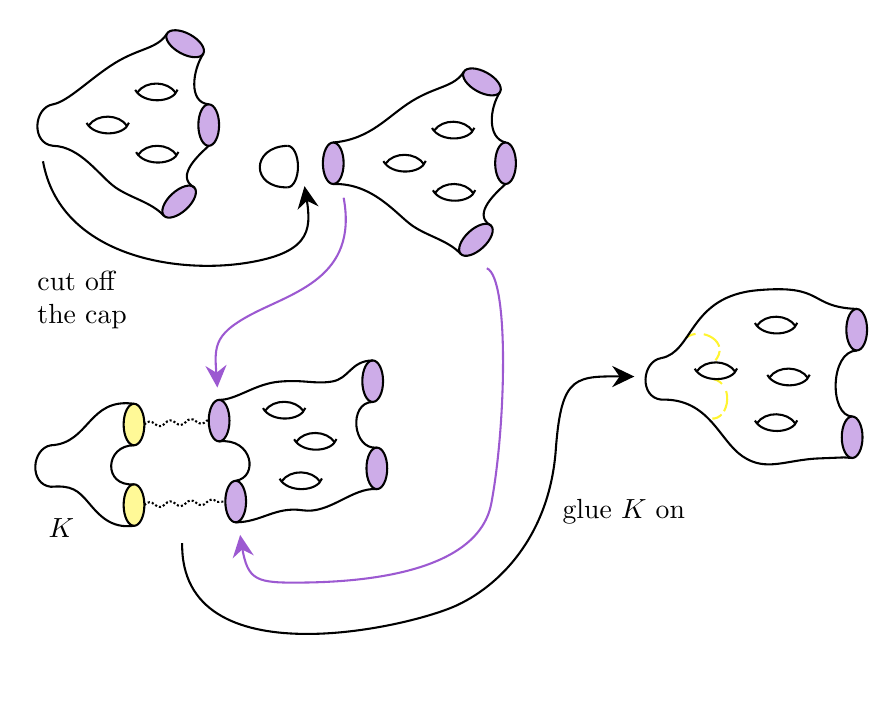
\begin{tikzpicture}[x=0.75pt,y=0.75pt,yscale=-1,xscale=1]
%uncomment if require: \path (0,366); %set diagram left start at 0, and has height of 366

%Curve Lines [id:da7456363211127895] 
\draw [color={rgb, 255:red, 255; green, 244; blue, 48 }  ,draw opacity=1 ] [dash pattern={on 3.75pt off 3pt on 7.5pt off 1.5pt}]  (325,164.55) .. controls (332.1,158.61) and (347.35,166.61) .. (338.45,176.18) ;
%Curve Lines [id:da21755327461639118] 
\draw [color={rgb, 255:red, 255; green, 244; blue, 48 }  ,draw opacity=1 ] [dash pattern={on 3.75pt off 3pt on 7.5pt off 1.5pt}]  (338,184.3) .. controls (349.35,186.86) and (345.2,206.93) .. (335.2,202.9) ;
%Shape: Ellipse [id:dp47766951388601575] 
\draw  [fill={rgb, 255:red, 255; green, 244; blue, 48 }  ,fill opacity=0.5 ] (54,206.28) .. controls (54,200.76) and (56.24,196.28) .. (59,196.28) .. controls (61.76,196.28) and (64,200.76) .. (64,206.28) .. controls (64,211.8) and (61.76,216.28) .. (59,216.28) .. controls (56.24,216.28) and (54,211.8) .. (54,206.28) -- cycle ;
%Shape: Ellipse [id:dp2213117305497102] 
\draw  [fill={rgb, 255:red, 255; green, 244; blue, 48 }  ,fill opacity=0.5 ] (54,245.08) .. controls (54,239.56) and (56.24,235.08) .. (59,235.08) .. controls (61.76,235.08) and (64,239.56) .. (64,245.08) .. controls (64,250.6) and (61.76,255.08) .. (59,255.08) .. controls (56.24,255.08) and (54,250.6) .. (54,245.08) -- cycle ;
%Curve Lines [id:da6254818543814082] 
\draw    (19,216.28) .. controls (37.64,215.38) and (36.83,193.28) .. (59,196.28) ;
%Curve Lines [id:da26678157319223816] 
\draw    (19,236.28) .. controls (28.93,235.48) and (31.92,237.86) .. (37.02,243.85) .. controls (42.11,249.84) and (47.65,256.53) .. (59,255.08) ;
%Curve Lines [id:da10195049737374684] 
\draw    (59,216.28) .. controls (44.83,216.28) and (43.83,236.28) .. (59,235.08) ;
%Curve Lines [id:da22082602480849645] 
\draw    (19,216.28) .. controls (9.6,217.81) and (8.27,235.15) .. (19,236.28) ;
%Shape: Ellipse [id:dp047839199679800104] 
\draw  [fill={rgb, 255:red, 156; green, 89; blue, 209 }  ,fill opacity=0.5 ] (229.04,36.82) .. controls (233.88,39.47) and (236.73,43.59) .. (235.4,46.01) .. controls (234.08,48.43) and (229.07,48.24) .. (224.23,45.59) .. controls (219.39,42.93) and (216.54,38.82) .. (217.87,36.4) .. controls (219.19,33.98) and (224.19,34.16) .. (229.04,36.82) -- cycle ;
%Shape: Ellipse [id:dp8497917036559762] 
\draw  [fill={rgb, 255:red, 156; green, 89; blue, 209 }  ,fill opacity=0.5 ] (233,80.4) .. controls (233,74.87) and (235.24,70.4) .. (238,70.4) .. controls (240.76,70.4) and (243,74.87) .. (243,80.4) .. controls (243,85.92) and (240.76,90.4) .. (238,90.4) .. controls (235.24,90.4) and (233,85.92) .. (233,80.4) -- cycle ;
%Curve Lines [id:da21030774171420585] 
\draw    (180.11,80.7) .. controls (184.19,74.66) and (194.93,75.04) .. (198.72,80.92) ;
%Curve Lines [id:da2054533399102827] 
\draw    (179.14,79.38) .. controls (183.14,86.42) and (197.45,85.74) .. (199.56,79.28) ;

%Curve Lines [id:da2922985882802336] 
\draw    (203.55,64.76) .. controls (207.63,58.71) and (218.37,59.1) .. (222.16,64.98) ;
%Curve Lines [id:da7481414220068059] 
\draw    (202.58,63.44) .. controls (206.58,70.47) and (220.89,69.8) .. (223,63.34) ;

%Curve Lines [id:da19338719689530326] 
\draw    (203.97,94.76) .. controls (208.05,88.71) and (218.79,89.1) .. (222.58,94.98) ;
%Curve Lines [id:da4856907558404082] 
\draw    (203,93.44) .. controls (207,100.47) and (221.32,99.8) .. (223.42,93.34) ;

%Shape: Ellipse [id:dp5786014847995782] 
\draw  [fill={rgb, 255:red, 156; green, 89; blue, 209 }  ,fill opacity=0.5 ] (227.13,120.96) .. controls (223.07,124.7) and (218.27,126.1) .. (216.39,124.07) .. controls (214.52,122.04) and (216.29,117.36) .. (220.35,113.61) .. controls (224.4,109.86) and (229.21,108.47) .. (231.08,110.5) .. controls (232.96,112.53) and (231.19,117.21) .. (227.13,120.96) -- cycle ;
%Curve Lines [id:da9074172955656375] 
\draw    (155,90.4) .. controls (174.15,89.85) and (185.51,105.16) .. (193,110.4) .. controls (200.49,115.63) and (210.39,117.55) .. (216.39,124.07) ;
%Curve Lines [id:da4486713212196154] 
\draw    (155,70.4) .. controls (173.15,68.85) and (181.21,57.63) .. (193,50.4) .. controls (204.79,43.17) and (213.13,43.77) .. (217.87,36.4) ;
%Curve Lines [id:da29408206197280085] 
\draw    (235.4,46.01) .. controls (230.2,54) and (229.05,68.15) .. (238,70.4) ;
%Curve Lines [id:da06937876092619744] 
\draw    (238,90.4) .. controls (234.2,94) and (221.2,105) .. (231.08,110.5) ;
%Shape: Ellipse [id:dp5834692450385205] 
\draw  [fill={rgb, 255:red, 156; green, 89; blue, 209 }  ,fill opacity=0.5 ] (86.04,18.42) .. controls (90.88,21.08) and (93.73,25.19) .. (92.4,27.62) .. controls (91.08,30.04) and (86.07,29.85) .. (81.23,27.19) .. controls (76.39,24.54) and (73.54,20.42) .. (74.87,18) .. controls (76.19,15.58) and (81.19,15.77) .. (86.04,18.42) -- cycle ;
%Shape: Ellipse [id:dp9981691356596056] 
\draw  [fill={rgb, 255:red, 156; green, 89; blue, 209 }  ,fill opacity=0.5 ] (90,62) .. controls (90,56.48) and (92.24,52) .. (95,52) .. controls (97.76,52) and (100,56.48) .. (100,62) .. controls (100,67.52) and (97.76,72) .. (95,72) .. controls (92.24,72) and (90,67.52) .. (90,62) -- cycle ;
%Curve Lines [id:da7930767734111239] 
\draw    (37.11,62.31) .. controls (41.19,56.26) and (51.93,56.65) .. (55.72,62.53) ;
%Curve Lines [id:da23296535928943463] 
\draw    (36.14,60.98) .. controls (40.14,68.02) and (54.45,67.35) .. (56.56,60.89) ;

%Curve Lines [id:da5658450019102096] 
\draw    (60.55,46.37) .. controls (64.63,40.32) and (75.37,40.7) .. (79.16,46.58) ;
%Curve Lines [id:da37655485995425364] 
\draw    (59.58,45.04) .. controls (63.58,52.08) and (77.89,51.4) .. (80,44.95) ;

%Curve Lines [id:da38704533910669703] 
\draw    (60.97,76.37) .. controls (65.05,70.32) and (75.79,70.7) .. (79.58,76.58) ;
%Curve Lines [id:da8417748691785382] 
\draw    (60,75.04) .. controls (64,82.08) and (78.32,81.4) .. (80.42,74.95) ;

%Shape: Ellipse [id:dp5782111136495405] 
\draw  [fill={rgb, 255:red, 156; green, 89; blue, 209 }  ,fill opacity=0.5 ] (84.13,102.56) .. controls (80.07,106.31) and (75.27,107.7) .. (73.39,105.67) .. controls (71.52,103.64) and (73.29,98.96) .. (77.35,95.21) .. controls (81.4,91.47) and (86.21,90.07) .. (88.08,92.1) .. controls (89.96,94.13) and (88.19,98.81) .. (84.13,102.56) -- cycle ;
%Curve Lines [id:da05841297602590634] 
\draw    (20,52) .. controls (10.6,53.53) and (9.27,70.87) .. (20,72) ;
%Curve Lines [id:da8590000152828204] 
\draw    (20,72) .. controls (33.24,72.25) and (42.51,86.77) .. (50,92) .. controls (57.49,97.23) and (67.39,99.15) .. (73.39,105.67) ;
%Curve Lines [id:da24903761379144307] 
\draw    (20,52) .. controls (27.34,50.67) and (38.21,39.23) .. (50,32) .. controls (61.79,24.77) and (70.13,25.37) .. (74.87,18) ;
%Curve Lines [id:da4778043785246958] 
\draw    (92.4,27.62) .. controls (87.2,35.6) and (85.05,51.15) .. (95,52) ;
%Curve Lines [id:da37177679505336103] 
\draw    (95,72) .. controls (91.2,75.6) and (78.2,86.6) .. (88.08,92.1) ;
%Curve Lines [id:da06243127894946254] 
\draw    (15.15,79.45) .. controls (23.15,124.45) and (78.05,133.95) .. (113.2,128.4) .. controls (146.42,123.16) and (144.4,110.63) .. (141.63,94.33) ;
\draw [shift={(141.15,91.45)}, rotate = 80.7] [fill={rgb, 255:red, 0; green, 0; blue, 0 }  ][line width=0.08]  [draw opacity=0] (10.72,-5.15) -- (0,0) -- (10.72,5.15) -- (7.12,0) -- cycle    ;
%Shape: Ellipse [id:dp8212226002047514] 
\draw  [fill={rgb, 255:red, 156; green, 89; blue, 209 }  ,fill opacity=0.5 ] (150,80.4) .. controls (150,74.87) and (152.24,70.4) .. (155,70.4) .. controls (157.76,70.4) and (160,74.87) .. (160,80.4) .. controls (160,85.92) and (157.76,90.4) .. (155,90.4) .. controls (152.24,90.4) and (150,85.92) .. (150,80.4) -- cycle ;
%Shape: Arc [id:dp4052834836534003] 
\draw  [draw opacity=0] (133,72) .. controls (133,72) and (133,72) .. (133,72) .. controls (133,72) and (133,72) .. (133,72) .. controls (135.76,72) and (138,76.48) .. (138,82) .. controls (138,87.52) and (135.76,92) .. (133,92) -- (133,82) -- cycle ; \draw   (133,72) .. controls (133,72) and (133,72) .. (133,72) .. controls (133,72) and (133,72) .. (133,72) .. controls (135.76,72) and (138,76.48) .. (138,82) .. controls (138,87.52) and (135.76,92) .. (133,92) ;  
%Curve Lines [id:da08409869661196623] 
\draw    (133,72) .. controls (115.15,72.45) and (115.15,92.45) .. (133,92) ;
%Curve Lines [id:da9204492733817433] 
\draw [color={rgb, 255:red, 156; green, 89; blue, 209 }  ,draw opacity=1 ]   (160,97) .. controls (167.17,135.65) and (135.35,142.65) .. (115.2,153.4) .. controls (96.16,163.56) and (97.79,169.48) .. (98.96,185.54) ;
\draw [shift={(99.15,188.45)}, rotate = 266.56] [fill={rgb, 255:red, 156; green, 89; blue, 209 }  ,fill opacity=1 ][line width=0.08]  [draw opacity=0] (10.72,-5.15) -- (0,0) -- (10.72,5.15) -- (7.12,0) -- cycle    ;
%Shape: Ellipse [id:dp776754946890608] 
\draw  [fill={rgb, 255:red, 156; green, 89; blue, 209 }  ,fill opacity=0.5 ] (95,204.4) .. controls (95,198.87) and (97.24,194.4) .. (100,194.4) .. controls (102.76,194.4) and (105,198.87) .. (105,204.4) .. controls (105,209.92) and (102.76,214.4) .. (100,214.4) .. controls (97.24,214.4) and (95,209.92) .. (95,204.4) -- cycle ;
%Shape: Ellipse [id:dp199266464828314] 
\draw  [fill={rgb, 255:red, 156; green, 89; blue, 209 }  ,fill opacity=0.5 ] (103,243.4) .. controls (103,237.87) and (105.24,233.4) .. (108,233.4) .. controls (110.76,233.4) and (113,237.87) .. (113,243.4) .. controls (113,248.92) and (110.76,253.4) .. (108,253.4) .. controls (105.24,253.4) and (103,248.92) .. (103,243.4) -- cycle ;
%Shape: Ellipse [id:dp645631326139301] 
\draw  [fill={rgb, 255:red, 156; green, 89; blue, 209 }  ,fill opacity=0.5 ] (169,185.4) .. controls (169,179.87) and (171.24,175.4) .. (174,175.4) .. controls (176.76,175.4) and (179,179.87) .. (179,185.4) .. controls (179,190.92) and (176.76,195.4) .. (174,195.4) .. controls (171.24,195.4) and (169,190.92) .. (169,185.4) -- cycle ;
%Shape: Ellipse [id:dp6611377988217855] 
\draw  [fill={rgb, 255:red, 156; green, 89; blue, 209 }  ,fill opacity=0.5 ] (171,227.4) .. controls (171,221.87) and (173.24,217.4) .. (176,217.4) .. controls (178.76,217.4) and (181,221.87) .. (181,227.4) .. controls (181,232.92) and (178.76,237.4) .. (176,237.4) .. controls (173.24,237.4) and (171,232.92) .. (171,227.4) -- cycle ;
%Curve Lines [id:da27596733021021924] 
\draw    (122.11,199.7) .. controls (126.19,193.66) and (136.93,194.04) .. (140.72,199.92) ;
%Curve Lines [id:da749269569119316] 
\draw    (121.14,198.38) .. controls (125.14,205.42) and (139.45,204.74) .. (141.56,198.28) ;

%Curve Lines [id:da4284732853055516] 
\draw    (137.11,214.7) .. controls (141.19,208.66) and (151.93,209.04) .. (155.72,214.92) ;
%Curve Lines [id:da23097840362923172] 
\draw    (136.14,213.38) .. controls (140.14,220.42) and (154.45,219.74) .. (156.56,213.28) ;

%Curve Lines [id:da208706920085994] 
\draw    (130.11,233.7) .. controls (134.19,227.66) and (144.93,228.04) .. (148.72,233.92) ;
%Curve Lines [id:da8277159491807085] 
\draw    (129.14,232.38) .. controls (133.14,239.42) and (147.45,238.74) .. (149.56,232.28) ;

%Curve Lines [id:da3865559692174718] 
\draw [color={rgb, 255:red, 156; green, 89; blue, 209 }  ,draw opacity=1 ]   (229,131) .. controls (239.93,135.66) and (238.15,207.25) .. (231.15,244.25) .. controls (224.15,281.25) and (157.2,282.4) .. (136.15,282.45) .. controls (116.05,282.5) and (113.27,280.36) .. (110.54,262.13) ;
\draw [shift={(110.15,259.45)}, rotate = 82.02] [fill={rgb, 255:red, 156; green, 89; blue, 209 }  ,fill opacity=1 ][line width=0.08]  [draw opacity=0] (10.72,-5.15) -- (0,0) -- (10.72,5.15) -- (7.12,0) -- cycle    ;
%Straight Lines [id:da364586372920236] 
\draw  [dash pattern={on 0.75pt off 0.75pt}]  (64,206.28) .. controls (65.57,204.51) and (67.23,204.41) .. (68.99,205.98) .. controls (70.76,207.54) and (72.42,207.44) .. (73.98,205.67) .. controls (75.54,203.9) and (77.2,203.8) .. (78.97,205.37) .. controls (80.74,206.94) and (82.4,206.84) .. (83.96,205.07) .. controls (85.52,203.3) and (87.18,203.2) .. (88.95,204.76) .. controls (90.72,206.33) and (92.38,206.23) .. (93.94,204.46) -- (95,204.4) -- (95,204.4) ;
%Straight Lines [id:da9532142435486358] 
\draw  [dash pattern={on 0.75pt off 0.75pt}]  (64,245.08) .. controls (65.59,243.35) and (67.26,243.28) .. (69,244.87) .. controls (70.74,246.46) and (72.4,246.39) .. (73.99,244.65) .. controls (75.58,242.91) and (77.25,242.84) .. (78.99,244.43) .. controls (80.72,246.02) and (82.39,245.95) .. (83.98,244.22) .. controls (85.57,242.48) and (87.24,242.41) .. (88.98,244) .. controls (90.71,245.59) and (92.38,245.52) .. (93.97,243.79) .. controls (95.56,242.05) and (97.23,241.98) .. (98.97,243.57) -- (103,243.4) -- (103,243.4) ;
%Curve Lines [id:da521532194512972] 
\draw    (100,194.4) .. controls (108.37,194.49) and (117.2,186.6) .. (129.2,185.6) .. controls (141.2,184.6) and (145.61,186.88) .. (154.2,185.6) .. controls (162.79,184.32) and (163.2,175.6) .. (174,175.4) ;
%Curve Lines [id:da6609977290169392] 
\draw    (100,214.4) .. controls (116.2,212.6) and (119.2,231.6) .. (108,233.4) ;
%Curve Lines [id:da995936588792983] 
\draw    (108,253.4) .. controls (120.2,253.4) and (127.2,245.6) .. (140.2,247.6) .. controls (153.2,249.6) and (164.14,236.46) .. (176,237.4) ;
%Curve Lines [id:da8490538991920554] 
\draw    (174,195.4) .. controls (162.2,195.6) and (164.2,218.6) .. (176,217.4) ;
%Curve Lines [id:da5179124360374171] 
\draw [color={rgb, 255:red, 0; green, 0; blue, 0 }  ,draw opacity=1 ]   (82.2,263.4) .. controls (81.2,329.4) and (192.05,304.15) .. (215.05,293.15) .. controls (238.05,282.15) and (259.35,257.05) .. (262.2,218.6) .. controls (264.95,181.5) and (271.57,182.99) .. (297.19,183.14) ;
\draw [shift={(300.05,183.15)}, rotate = 180] [fill={rgb, 255:red, 0; green, 0; blue, 0 }  ,fill opacity=1 ][line width=0.08]  [draw opacity=0] (10.72,-5.15) -- (0,0) -- (10.72,5.15) -- (7.12,0) -- cycle    ;
%Curve Lines [id:da9066189595509849] 
\draw    (313,174.28) .. controls (303.6,175.81) and (302.27,193.15) .. (313,194.28) ;
%Shape: Ellipse [id:dp1720032696838898] 
\draw  [fill={rgb, 255:red, 156; green, 89; blue, 209 }  ,fill opacity=0.5 ] (402.2,160.6) .. controls (402.2,155.08) and (404.44,150.6) .. (407.2,150.6) .. controls (409.96,150.6) and (412.2,155.08) .. (412.2,160.6) .. controls (412.2,166.12) and (409.96,170.6) .. (407.2,170.6) .. controls (404.44,170.6) and (402.2,166.12) .. (402.2,160.6) -- cycle ;
%Shape: Ellipse [id:dp5828118842225084] 
\draw  [fill={rgb, 255:red, 156; green, 89; blue, 209 }  ,fill opacity=0.5 ] (400,212.4) .. controls (400,206.87) and (402.24,202.4) .. (405,202.4) .. controls (407.76,202.4) and (410,206.87) .. (410,212.4) .. controls (410,217.92) and (407.76,222.4) .. (405,222.4) .. controls (402.24,222.4) and (400,217.92) .. (400,212.4) -- cycle ;
%Curve Lines [id:da12748011779331514] 
\draw    (359.11,158.7) .. controls (363.19,152.66) and (373.93,153.04) .. (377.72,158.92) ;
%Curve Lines [id:da6587047534533921] 
\draw    (358.14,157.38) .. controls (362.14,164.42) and (376.45,163.74) .. (378.56,157.28) ;

%Curve Lines [id:da37914622908130136] 
\draw    (365.11,183.7) .. controls (369.19,177.66) and (379.93,178.04) .. (383.72,183.92) ;
%Curve Lines [id:da09849809070853266] 
\draw    (364.14,182.38) .. controls (368.14,189.42) and (382.45,188.74) .. (384.56,182.28) ;

%Curve Lines [id:da7128015832866221] 
\draw    (359.11,205.7) .. controls (363.19,199.66) and (373.93,200.04) .. (377.72,205.92) ;
%Curve Lines [id:da443803466114602] 
\draw    (358.14,204.38) .. controls (362.14,211.42) and (376.45,210.74) .. (378.56,204.28) ;

%Curve Lines [id:da9774803119180495] 
\draw    (330.11,180.7) .. controls (334.19,174.66) and (344.93,175.04) .. (348.72,180.92) ;
%Curve Lines [id:da010681509366633035] 
\draw    (329.14,179.38) .. controls (333.14,186.42) and (347.45,185.74) .. (349.56,179.28) ;

%Curve Lines [id:da8204011461116862] 
\draw    (313,194.28) .. controls (336.2,193.6) and (340.77,213.84) .. (352.2,221.6) .. controls (363.63,229.36) and (372.89,223.22) .. (389.2,222.6) .. controls (405.51,221.98) and (398.97,222.05) .. (405,222.4) ;
%Curve Lines [id:da13590361013687124] 
\draw    (313,174.28) .. controls (328.63,171.43) and (326.2,144.6) .. (359.2,141.6) .. controls (392.2,138.6) and (383.4,149.6) .. (407.2,150.6) ;
%Curve Lines [id:da4501000826918429] 
\draw    (407.2,170.6) .. controls (394.05,171.15) and (394.05,202.15) .. (405,202.4) ;

% Text Node
\draw (24.06,256.28) node    {$K$};
% Text Node
\draw (264,240.8) node [anchor=north west][inner sep=0.75pt]   [align=left] {glue $\displaystyle K$ on};
% Text Node
\draw (11,131) node [anchor=north west][inner sep=0.75pt]   [align=left] {cut off \\the cap };


\end{tikzpicture}

        \caption{An \( \omega_{g,n}\) having a cap removed before being glued to \(K\) to increase the genus.}
        \label{fig:trcut}
    \end{figure}
    
    Visually, imagine setting the width of the tubes in the picture to zero, to produce graphs of various genus, where a boundary becomes an external vertex in the graph, and the genus of the blob matches the genus of the graph. Also consider the cap as a specially labelled external vertex or a root. Of course, there is a potential ambiguity, there are multiple graphs of genus \(g\). One constraint that will need to be imposed is that all internal vertices will be degree \(3\). Then instead of a single graph, it will then be the case that \(\omega_{g,n}\) is decomposed into a weighted sum of these possible options. For example figure (\ref{fig:trprim}), \( \omega_{2,3}\) will correspond to a sum of these graphs plus permutations. These graphs are distinct from the graphical sums considered usually for topological recursion \cite{eynard_orantin}. Airy structures will describe this procedure. 
    \begin{figure}[!htb]
        \centering 
        

\tikzset{every picture/.style={line width=0.75pt}} %set default line width to 0.75pt        

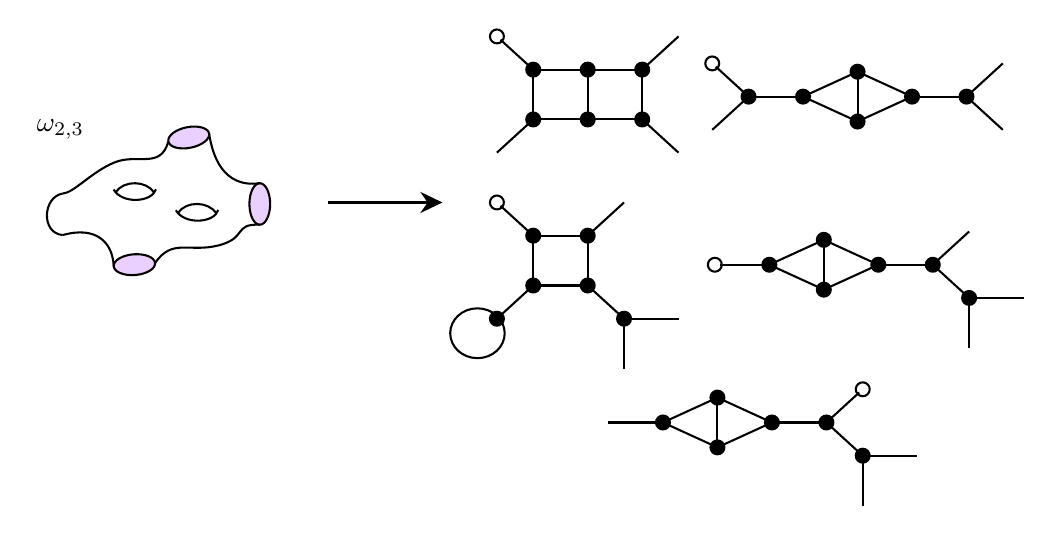
\begin{tikzpicture}[x=0.75pt,y=0.75pt,yscale=-1,xscale=1]
%uncomment if require: \path (0,261); %set diagram left start at 0, and has height of 261

%Straight Lines [id:da5122725041953835] 
\draw    (273.75,55) -- (300,55) ;
\draw [shift={(300,55)}, rotate = 0] [color={rgb, 255:red, 0; green, 0; blue, 0 }  ][fill={rgb, 255:red, 0; green, 0; blue, 0 }  ][line width=0.75]      (0, 0) circle [x radius= 3.35, y radius= 3.35]   ;
\draw [shift={(273.75,55)}, rotate = 0] [color={rgb, 255:red, 0; green, 0; blue, 0 }  ][fill={rgb, 255:red, 0; green, 0; blue, 0 }  ][line width=0.75]      (0, 0) circle [x radius= 3.35, y radius= 3.35]   ;
%Straight Lines [id:da28474322327009105] 
\draw    (273.75,31) -- (300,31) ;
\draw [shift={(300,31)}, rotate = 0] [color={rgb, 255:red, 0; green, 0; blue, 0 }  ][fill={rgb, 255:red, 0; green, 0; blue, 0 }  ][line width=0.75]      (0, 0) circle [x radius= 3.35, y radius= 3.35]   ;
\draw [shift={(273.75,31)}, rotate = 0] [color={rgb, 255:red, 0; green, 0; blue, 0 }  ][fill={rgb, 255:red, 0; green, 0; blue, 0 }  ][line width=0.75]      (0, 0) circle [x radius= 3.35, y radius= 3.35]   ;
%Straight Lines [id:da10829389002897793] 
\draw    (300,31) -- (326.25,31) ;
%Straight Lines [id:da2680222353656253] 
\draw    (300,31) -- (300,55) ;
%Straight Lines [id:da3878078948480259] 
\draw    (273.75,31) -- (273.75,55) ;
%Straight Lines [id:da8964050542040451] 
\draw    (343.75,15) -- (326.25,31) ;
%Straight Lines [id:da2090118876269007] 
\draw    (326.25,55) -- (300,55) ;
%Straight Lines [id:da7172980906443349] 
\draw    (326.25,31) -- (326.25,55) ;
\draw [shift={(326.25,55)}, rotate = 90] [color={rgb, 255:red, 0; green, 0; blue, 0 }  ][fill={rgb, 255:red, 0; green, 0; blue, 0 }  ][line width=0.75]      (0, 0) circle [x radius= 3.35, y radius= 3.35]   ;
\draw [shift={(326.25,31)}, rotate = 90] [color={rgb, 255:red, 0; green, 0; blue, 0 }  ][fill={rgb, 255:red, 0; green, 0; blue, 0 }  ][line width=0.75]      (0, 0) circle [x radius= 3.35, y radius= 3.35]   ;
%Straight Lines [id:da8298682809994327] 
\draw    (343.75,71) -- (326.25,55) ;
%Straight Lines [id:da7340542571833397] 
\draw    (273.75,135) -- (256.25,151) ;
\draw [shift={(256.25,151)}, rotate = 137.56] [color={rgb, 255:red, 0; green, 0; blue, 0 }  ][fill={rgb, 255:red, 0; green, 0; blue, 0 }  ][line width=0.75]      (0, 0) circle [x radius= 3.35, y radius= 3.35]   ;
\draw [shift={(273.75,135)}, rotate = 137.56] [color={rgb, 255:red, 0; green, 0; blue, 0 }  ][fill={rgb, 255:red, 0; green, 0; blue, 0 }  ][line width=0.75]      (0, 0) circle [x radius= 3.35, y radius= 3.35]   ;
%Shape: Ellipse [id:dp8951997570910564] 
\draw   (233.75,158) .. controls (233.75,151.37) and (239.63,146) .. (246.88,146) .. controls (254.12,146) and (260,151.37) .. (260,158) .. controls (260,164.63) and (254.12,170) .. (246.88,170) .. controls (239.63,170) and (233.75,164.63) .. (233.75,158) -- cycle ;
%Straight Lines [id:da30041493250608486] 
\draw    (273.75,135) -- (273.75,111) ;
\draw [shift={(273.75,111)}, rotate = 270] [color={rgb, 255:red, 0; green, 0; blue, 0 }  ][fill={rgb, 255:red, 0; green, 0; blue, 0 }  ][line width=0.75]      (0, 0) circle [x radius= 3.35, y radius= 3.35]   ;
%Straight Lines [id:da06815777790639788] 
\draw    (273.75,135) -- (300,135) ;
\draw [shift={(300,135)}, rotate = 0] [color={rgb, 255:red, 0; green, 0; blue, 0 }  ][fill={rgb, 255:red, 0; green, 0; blue, 0 }  ][line width=0.75]      (0, 0) circle [x radius= 3.35, y radius= 3.35]   ;
%Straight Lines [id:da39270668609938153] 
\draw    (273.75,111) -- (300,111) ;
%Straight Lines [id:da7632138968433353] 
\draw    (300,111) -- (300,135) ;
\draw [shift={(300,111)}, rotate = 90] [color={rgb, 255:red, 0; green, 0; blue, 0 }  ][fill={rgb, 255:red, 0; green, 0; blue, 0 }  ][line width=0.75]      (0, 0) circle [x radius= 3.35, y radius= 3.35]   ;
%Straight Lines [id:da5129578501641567] 
\draw    (300,135) -- (317.5,151) ;
%Straight Lines [id:da3795104652375495] 
\draw    (317.5,151) -- (317.5,175) ;
%Straight Lines [id:da36668627460221803] 
\draw    (317.5,151) -- (343.75,151) ;
\draw [shift={(317.5,151)}, rotate = 0] [color={rgb, 255:red, 0; green, 0; blue, 0 }  ][fill={rgb, 255:red, 0; green, 0; blue, 0 }  ][line width=0.75]      (0, 0) circle [x radius= 3.35, y radius= 3.35]   ;
%Straight Lines [id:da04810774235669735] 
\draw    (257.98,96.59) -- (273.75,111) ;
\draw [shift={(256.25,95)}, rotate = 42.44] [color={rgb, 255:red, 0; green, 0; blue, 0 }  ][line width=0.75]      (0, 0) circle [x radius= 3.35, y radius= 3.35]   ;
%Straight Lines [id:da3040121567882321] 
\draw    (273.75,55) -- (256.25,71) ;
%Straight Lines [id:da8929796050220722] 
\draw    (257.98,16.59) -- (273.75,31) ;
\draw [shift={(256.25,15)}, rotate = 42.44] [color={rgb, 255:red, 0; green, 0; blue, 0 }  ][line width=0.75]      (0, 0) circle [x radius= 3.35, y radius= 3.35]   ;
%Straight Lines [id:da6909706145423474] 
\draw    (300,111) -- (317.5,95) ;
%Straight Lines [id:da23015717978846162] 
\draw    (430,32) -- (430,56) ;
\draw [shift={(430,56)}, rotate = 90] [color={rgb, 255:red, 0; green, 0; blue, 0 }  ][fill={rgb, 255:red, 0; green, 0; blue, 0 }  ][line width=0.75]      (0, 0) circle [x radius= 3.35, y radius= 3.35]   ;
\draw [shift={(430,32)}, rotate = 90] [color={rgb, 255:red, 0; green, 0; blue, 0 }  ][fill={rgb, 255:red, 0; green, 0; blue, 0 }  ][line width=0.75]      (0, 0) circle [x radius= 3.35, y radius= 3.35]   ;
%Straight Lines [id:da218526175596091] 
\draw    (403.75,44) -- (430,32) ;
%Straight Lines [id:da4625716861489917] 
\draw    (403.75,44) -- (430,56) ;
%Straight Lines [id:da7692276877958857] 
\draw    (430,56) -- (456.25,44) ;
%Straight Lines [id:da8311350234486945] 
\draw    (430,32) -- (456.25,44) ;
%Straight Lines [id:da22531345274551862] 
\draw    (377.5,44) -- (403.75,44) ;
\draw [shift={(403.75,44)}, rotate = 0] [color={rgb, 255:red, 0; green, 0; blue, 0 }  ][fill={rgb, 255:red, 0; green, 0; blue, 0 }  ][line width=0.75]      (0, 0) circle [x radius= 3.35, y radius= 3.35]   ;
\draw [shift={(377.5,44)}, rotate = 0] [color={rgb, 255:red, 0; green, 0; blue, 0 }  ][fill={rgb, 255:red, 0; green, 0; blue, 0 }  ][line width=0.75]      (0, 0) circle [x radius= 3.35, y radius= 3.35]   ;
%Straight Lines [id:da5091038921692058] 
\draw    (456.25,44) -- (482.5,44) ;
\draw [shift={(482.5,44)}, rotate = 0] [color={rgb, 255:red, 0; green, 0; blue, 0 }  ][fill={rgb, 255:red, 0; green, 0; blue, 0 }  ][line width=0.75]      (0, 0) circle [x radius= 3.35, y radius= 3.35]   ;
\draw [shift={(456.25,44)}, rotate = 0] [color={rgb, 255:red, 0; green, 0; blue, 0 }  ][fill={rgb, 255:red, 0; green, 0; blue, 0 }  ][line width=0.75]      (0, 0) circle [x radius= 3.35, y radius= 3.35]   ;
%Straight Lines [id:da8664330260674795] 
\draw    (361.73,29.59) -- (377.5,44) ;
\draw [shift={(360,28)}, rotate = 42.44] [color={rgb, 255:red, 0; green, 0; blue, 0 }  ][line width=0.75]      (0, 0) circle [x radius= 3.35, y radius= 3.35]   ;
%Straight Lines [id:da3192935693014617] 
\draw    (377.5,44) -- (360,60) ;
%Straight Lines [id:da4798044818656505] 
\draw    (500,28) -- (482.5,44) ;
%Straight Lines [id:da5438422167321475] 
\draw    (482.5,44) -- (500,60) ;
%Straight Lines [id:da1919924062947258] 
\draw    (413.75,113) -- (413.75,137) ;
\draw [shift={(413.75,137)}, rotate = 90] [color={rgb, 255:red, 0; green, 0; blue, 0 }  ][fill={rgb, 255:red, 0; green, 0; blue, 0 }  ][line width=0.75]      (0, 0) circle [x radius= 3.35, y radius= 3.35]   ;
\draw [shift={(413.75,113)}, rotate = 90] [color={rgb, 255:red, 0; green, 0; blue, 0 }  ][fill={rgb, 255:red, 0; green, 0; blue, 0 }  ][line width=0.75]      (0, 0) circle [x radius= 3.35, y radius= 3.35]   ;
%Straight Lines [id:da8465955727425204] 
\draw    (387.5,125) -- (413.75,113) ;
%Straight Lines [id:da6806428111346395] 
\draw    (387.5,125) -- (413.75,137) ;
%Straight Lines [id:da6919470348796317] 
\draw    (413.75,137) -- (440,125) ;
%Straight Lines [id:da2467178879862778] 
\draw    (413.75,113) -- (440,125) ;
%Straight Lines [id:da10206442403366411] 
\draw    (363.6,125) -- (387.5,125) ;
\draw [shift={(387.5,125)}, rotate = 0] [color={rgb, 255:red, 0; green, 0; blue, 0 }  ][fill={rgb, 255:red, 0; green, 0; blue, 0 }  ][line width=0.75]      (0, 0) circle [x radius= 3.35, y radius= 3.35]   ;
\draw [shift={(361.25,125)}, rotate = 0] [color={rgb, 255:red, 0; green, 0; blue, 0 }  ][line width=0.75]      (0, 0) circle [x radius= 3.35, y radius= 3.35]   ;
%Straight Lines [id:da24121818086261326] 
\draw    (466.25,125) -- (440,125) ;
\draw [shift={(440,125)}, rotate = 180] [color={rgb, 255:red, 0; green, 0; blue, 0 }  ][fill={rgb, 255:red, 0; green, 0; blue, 0 }  ][line width=0.75]      (0, 0) circle [x radius= 3.35, y radius= 3.35]   ;
%Straight Lines [id:da07657668079543134] 
\draw    (466.25,125) -- (483.75,141) ;
%Straight Lines [id:da7280856830918088] 
\draw    (483.75,109) -- (466.25,125) ;
\draw [shift={(466.25,125)}, rotate = 137.56] [color={rgb, 255:red, 0; green, 0; blue, 0 }  ][fill={rgb, 255:red, 0; green, 0; blue, 0 }  ][line width=0.75]      (0, 0) circle [x radius= 3.35, y radius= 3.35]   ;
%Straight Lines [id:da14505738593155804] 
\draw    (483.75,141) -- (483.75,165) ;
\draw [shift={(483.75,141)}, rotate = 90] [color={rgb, 255:red, 0; green, 0; blue, 0 }  ][fill={rgb, 255:red, 0; green, 0; blue, 0 }  ][line width=0.75]      (0, 0) circle [x radius= 3.35, y radius= 3.35]   ;
%Straight Lines [id:da9161411663684729] 
\draw    (483.75,141) -- (510,141) ;
%Shape: Ellipse [id:dp9983240440491878] 
\draw  [fill={rgb, 255:red, 144; green, 19; blue, 254 }  ,fill opacity=0.2 ] (106.81,58.78) .. controls (112.23,57.72) and (117.06,59.05) .. (117.59,61.76) .. controls (118.12,64.47) and (114.16,67.53) .. (108.74,68.59) .. controls (103.32,69.66) and (98.5,68.32) .. (97.96,65.62) .. controls (97.43,62.91) and (101.39,59.85) .. (106.81,58.78) -- cycle ;
%Shape: Ellipse [id:dp8744151668416713] 
\draw  [fill={rgb, 255:red, 144; green, 19; blue, 254 }  ,fill opacity=0.2 ] (137,95.71) .. controls (137,90.19) and (139.24,85.71) .. (142,85.71) .. controls (144.76,85.71) and (147,90.19) .. (147,95.71) .. controls (147,101.23) and (144.76,105.71) .. (142,105.71) .. controls (139.24,105.71) and (137,101.23) .. (137,95.71) -- cycle ;
%Curve Lines [id:da2869657736144847] 
\draw    (72.55,90.08) .. controls (76.63,84.03) and (87.37,84.41) .. (91.16,90.29) ;
%Curve Lines [id:da47401693953711166] 
\draw    (71.58,88.75) .. controls (75.58,95.79) and (89.89,95.11) .. (92,88.65) ;

%Curve Lines [id:da32566055187581266] 
\draw    (102.55,100.08) .. controls (106.63,94.03) and (117.37,94.41) .. (121.16,100.29) ;
%Curve Lines [id:da2019919284274363] 
\draw    (101.58,98.75) .. controls (105.58,105.79) and (119.89,105.11) .. (122,98.65) ;

%Shape: Ellipse [id:dp5907492416219241] 
\draw  [fill={rgb, 255:red, 144; green, 19; blue, 254 }  ,fill opacity=0.2 ] (81.97,129.94) .. controls (76.46,130.37) and (71.83,128.48) .. (71.62,125.72) .. controls (71.4,122.97) and (75.69,120.39) .. (81.2,119.97) .. controls (86.71,119.55) and (91.34,121.43) .. (91.56,124.19) .. controls (91.77,126.94) and (87.48,129.52) .. (81.97,129.94) -- cycle ;
%Curve Lines [id:da9618686062811871] 
\draw    (47,90.71) .. controls (37.6,92.24) and (36.27,109.58) .. (47,110.71) ;
%Curve Lines [id:da9315086155026743] 
\draw    (47,90.71) .. controls (52.46,90.41) and (60.85,80.26) .. (72,75.71) .. controls (83.15,71.16) and (94.15,79.16) .. (97.96,65.62) ;
%Curve Lines [id:da26002550218872766] 
\draw    (117.59,61.76) .. controls (119.15,72.16) and (124.15,88.16) .. (142,85.71) ;
%Curve Lines [id:da07750632050652662] 
\draw    (47,110.71) .. controls (63.15,106.16) and (71.15,114.16) .. (71.62,125.72) ;
%Straight Lines [id:da05033777354261337] 
\draw    (175,95) -- (227,95) ;
\draw [shift={(230,95)}, rotate = 180] [fill={rgb, 255:red, 0; green, 0; blue, 0 }  ][line width=0.08]  [draw opacity=0] (10.72,-5.15) -- (0,0) -- (10.72,5.15) -- (7.12,0) -- cycle    ;
%Curve Lines [id:da9997148036675941] 
\draw    (91.56,124.19) .. controls (99.83,112.04) and (107.85,119.26) .. (122,115.71) .. controls (136.15,112.16) and (129.15,105.16) .. (142,105.71) ;
%Straight Lines [id:da9155663136556371] 
\draw    (362.5,189) -- (362.5,213) ;
\draw [shift={(362.5,213)}, rotate = 90] [color={rgb, 255:red, 0; green, 0; blue, 0 }  ][fill={rgb, 255:red, 0; green, 0; blue, 0 }  ][line width=0.75]      (0, 0) circle [x radius= 3.35, y radius= 3.35]   ;
\draw [shift={(362.5,189)}, rotate = 90] [color={rgb, 255:red, 0; green, 0; blue, 0 }  ][fill={rgb, 255:red, 0; green, 0; blue, 0 }  ][line width=0.75]      (0, 0) circle [x radius= 3.35, y radius= 3.35]   ;
%Straight Lines [id:da6144740353067586] 
\draw    (336.25,201) -- (362.5,189) ;
%Straight Lines [id:da731979461617581] 
\draw    (336.25,201) -- (362.5,213) ;
%Straight Lines [id:da3021389190911925] 
\draw    (362.5,213) -- (388.75,201) ;
%Straight Lines [id:da3499524614238886] 
\draw    (362.5,189) -- (388.75,201) ;
%Straight Lines [id:da7267547149941356] 
\draw    (310,201) -- (336.25,201) ;
\draw [shift={(336.25,201)}, rotate = 0] [color={rgb, 255:red, 0; green, 0; blue, 0 }  ][fill={rgb, 255:red, 0; green, 0; blue, 0 }  ][line width=0.75]      (0, 0) circle [x radius= 3.35, y radius= 3.35]   ;
%Straight Lines [id:da358756631970491] 
\draw    (415,201) -- (388.75,201) ;
\draw [shift={(388.75,201)}, rotate = 180] [color={rgb, 255:red, 0; green, 0; blue, 0 }  ][fill={rgb, 255:red, 0; green, 0; blue, 0 }  ][line width=0.75]      (0, 0) circle [x radius= 3.35, y radius= 3.35]   ;
%Straight Lines [id:da24810710585260554] 
\draw    (415,201) -- (432.5,217) ;
%Straight Lines [id:da6217625759194046] 
\draw    (430.77,186.59) -- (415,201) ;
\draw [shift={(415,201)}, rotate = 137.56] [color={rgb, 255:red, 0; green, 0; blue, 0 }  ][fill={rgb, 255:red, 0; green, 0; blue, 0 }  ][line width=0.75]      (0, 0) circle [x radius= 3.35, y radius= 3.35]   ;
\draw [shift={(432.5,185)}, rotate = 137.56] [color={rgb, 255:red, 0; green, 0; blue, 0 }  ][line width=0.75]      (0, 0) circle [x radius= 3.35, y radius= 3.35]   ;
%Straight Lines [id:da10367763599277802] 
\draw    (432.5,217) -- (432.5,241) ;
\draw [shift={(432.5,217)}, rotate = 90] [color={rgb, 255:red, 0; green, 0; blue, 0 }  ][fill={rgb, 255:red, 0; green, 0; blue, 0 }  ][line width=0.75]      (0, 0) circle [x radius= 3.35, y radius= 3.35]   ;
%Straight Lines [id:da19412967587984997] 
\draw    (432.5,217) -- (458.75,217) ;

% Text Node
\draw (46,59.71) node    {$\omega _{2,3}$};


\end{tikzpicture}

        \caption{Primitives for \( \omega_{2,3}\). In particular the graphs will correspond to coefficients of the function \( S_{2,3}(x)\) in chapter (\ref{chapter:airy}). The vertex connected to the unfilled circle is the root.}
        \label{fig:trprim}
    \end{figure}

    

    \begin{lem}[\cite{eynard_orantin}]
    \( \omega_{g,n}(p_1,\dots,p_n)\) are symmetric under permutations of the \(p_i\), where \( p_i\) coordinate on \( \Sigma\).
    \end{lem}
    This was originally proven by Eynard Orantin, but this will also be provable from the Airy structure perspective.
    
    A closely related object to the \( \omega_{g,n}\) are the \emph{symplectic invariants}:
    
    \begin{defn}[Symplectic invariants]
    \[ F_g = \sum_{\alpha \in R} \Res_{z=\alpha}(\varphi(p) \omega_{g,1}(p) ),\]
    where \( \varphi(p)\) is a locally defined function so \( d \varphi(p) = \omega_{0,1}(p)\).
    \end{defn}

    These appear in chapter (\ref{chapter:Atensor}). \(F_g\) are called symplectic invariants because they are conjectured to be invariant under a change of the \( (x,y)\) of the form
    \[ ( x, y ) \rightarrow ( a \,x + b\, y, c\, x + d \,y ). \] 
    where 
    \[ \left( \begin{array}{cc}
         a & b   \\
         c & d 
    \end{array} \right) \in \mathrm{SL}(2, \mathbb{R} ). \]
    Furthermore, they are independent of the foliation.
    
    \begin{ex}[An elliptic curve]
    Let \( \tau \) be a complex number in the upper half plane. Define \(\wp(z)\), \emph{Weierstrass's elliptic function} \cite{whitwhat} by 
    \[ \wp(z) = \frac{1}{z^2} + \sum_{\overset{m,n \in \mathbb{Z}
    }{ m^2 + n^2 \neq 0}} \left( \frac{1}{(z+m+n \tau)^2} -\frac{1}{(m+n \tau)^2}    \right).\] 
    Define \( x(z) = \wp(z) \), \(y(z) = \wp'(z)\). The Bergman kernel is given by
    \[  B(z_1,z_2) = \wp(z_1-z_2) + c(\tau) \,dz_1 dz_2,\]
    where \( c(\tau)\) is chosen so \(a\)-periods vanish.
    \( x\) and \(y\) can be shown to satisfy a polynomial equation of the form 
    \[ y^2 = 4 x^3 + g_2 x + g_3,\]
    where \(g_2\) and \(g_3 \in \mathbb{C}\) depend on \( \tau\).
    This defines a spectral curve \( (\Sigma, x,y,B)\), where \(\Sigma\) is a complex torus \( \mathbb{C}/\Lambda\), where \( \Lambda\) is a lattice in \( \mathbb{C}\), \( \Lambda = \mathbb{Z} + \tau \mathbb{Z} \).
    \end{ex}
    

    \section{Poisson schemes}
    Recall the definition of a Poisson algebra  \cite{jordan}:

    \begin{defn}[Poisson algebra]
            Let \( \mathbf{k} \) be a field. A \emph{Poisson algebra}, \(P\), is an associative \( \mathbf{k} \)-algebra, equipped with an extra operation called the \emph{Poisson bracket}, \( \{ \cdot  , \cdot  \} : P \otimes_{\mathbf{k}} P \rightarrow P\). The Poisson bracket is bilinear,
            anti-symmetric, alternating, satisfies the \emph{Jacobi identity}:
            \[ \{ f, \{g,h\} \} +\{ h, \{f,g\}\} + \{ g ,\{h,f\}\} = 0\] 
            and the \emph{Leibniz rule}:
            \[ \{ f, g \cdot h \} = \{f,g\}\cdot h + g \cdot \{ f , h\}.\]
    \end{defn}
    
    \begin{defn}[Poisson scheme]
        A scheme \((X, \mathcal{O}_X)\) is \emph{Poisson} if \( \mathcal{O}_X\) is a sheaf of Poisson algebras.
    \end{defn}
    
    Consider a Poisson variety \( (X,\mathcal{O}_X)\) and a genus \(g\) curve \(\Sigma\) inside \( X\), so \( \Sigma \rightarrow X\). 
    
    
    Let \( \mathcal{B}\) be the deformation space of \( \Sigma\) inside \(X\).  The cohomology group \[ H^0(\Sigma, \nu_\Sigma) \cong H^0( \Sigma, K_\Sigma) \cong \mathbb{C}^g \]
    where \( \nu_\Sigma\) is the conormal sheaf, gives first order deformations of \(\Sigma\) in \(X\). For example, Nishinou proves that any first order deformation can be lifted to any higher order deformations, so deformations are unobstructed \cite{nishi_obs}. Then \( \mathcal{B}\) is a smooth deformation space, of dimension \(g\), where the tangent space at a point \(\Sigma\) in \( \mathcal{B}\) can be identified with the cohomology group:
    \[T_\Sigma \mathcal{B} \cong H^0(\Sigma, \nu_\Sigma).\]
    Note that obstructions live in the cohomology group \(H^1(\Sigma, \nu_\Sigma)\),
    \[ H^1( \Sigma ,\nu_\Sigma) \cong H^1(\Sigma, K_\Sigma) \cong \mathbb{C} \neq 0. \]
    Trivial \(H^1(\Sigma ,\nu_\Sigma)\) would immediately give unobstructed deformations. In this case however, we can use, for example \cite{nishi_obs}, to show there are extra conditions, which gives unobstructed deformations.
        %canonical sheaf \( K_X\)
        
    Further we have the isomorphism 
    \[  H^0(\Sigma, \nu_\Sigma) \cong H^{0}(\Sigma, K_\Sigma),\] 
    by the adjunction formula:
    \[ K_\Sigma \cong K_{X/\Sigma} \otimes \nu_\Sigma \cong \nu_\Sigma. \]
    %where we call \(   H^{0}(\Sigma, K_\Sigma)\) the space of holomorphic differentials on \( \Sigma\).
    %The deformation space \( \mathcal{B}\) is a dimension \(g\) moduli space. 
    
    A particular case of interest is when \(\Sigma \rightarrow  X\), where \(X = T^{*}S\) is the cotangent bundle of an algebraic surface \(S\). \(X\) is naturally equipped with a symplectic form, and singular points of the symplectic form define a divisor.

    %Over \( \mathcal{B}\) we are interested in constructing a bundle or sheaf \( \mathcal{H}\) equipped with a connection. In the symplectic case the connection on \( \mathcal{H}\) is the Gauss-Manin connection.


    %theorem 
    
    %
    \section{An example Airy structure in finite dimensions}
    \label{sec:finiteexintro}
    Let \( \mathbf{k}\) be a field of characteristic zero. Kontsevich and Soibelman formulated topological recursion in terms of an \emph{Airy structure} \cite{ks_airy, abcd, airy_semisimple, eynard_abc}. Consider a \emph{\hyperref[defn:symplectic]{symplectic vector space}} \((W,\omega)\). An \hyperref[defn:airystruct]{Airy structure} characterises a \emph{quadratic Lagrangian} subvariety \(\mathbb{L}\) in \(W\). Quadratic means \( \mathbb{L}\) is defined by a collection of polynomials of degree \(\leq 2\). Note \(W\) has identified with a symplectic affine space.
    %The definition applies in both finite and infinite dimensions. Associated to the tangent space of \( \mathbb{L}\), \(L= \mathcal{T}_0 \mathbb{L}\), 
    
    
    %identify affine space and W
    
    \begin{ex} 
    \label{ex:introconic}
    Consider the complex conic \( \mathbb{L}\) in \( \mathbb{A}^2\) defined by the ideal:
    \[I(\mathbb{L})=\langle-y+a\,x^2+2\,b\,x\,y+c\,y^2\rangle,\]
    so
    \[ \mathbb{L}  = \Spec\left( \frac{\mathbb{C}[x,y]}{I(\mathbb{L})} \right).\] 
    \(\mathbb{L}\) is a quadratic Lagrangian subvariety in the symplectic affine space \(W \cong \mathbb{A}^2 \)
    \end{ex} 
    
    
    Example (\ref{ex:introconic}) is more fully investigated in chapter (\ref{chapter:deformation}), and provides interesting insight into the more general problem. For generating the topological recursion invariants however, \(W\) must be infinite dimensional. We consider a \(2N\)-dimensional analog first to give an overview of Airy structures.
    
    Consider a finite-dimensional symplectic space \((W\cong \mathbf{k}^{2N}, \omega ) \), and a quadratic Lagrangian subvariety \(\mathbb{L} \subset W \cong \mathbb{A}^{2N} = \Spec( \mathbf{k}[x_1, \dots ,x_N, y_1, \dots, y_N])\), with a Zariski tangent space \( L=\mathcal{T}_0\mathbb{L} \subset W \).  Note the identification of points in \(W\) with an affine space.
    
    Pick a complement \(V\) to \(L\) in \(W\), so
    \(W \cong L\oplus V.\)
    Then observe that the exact sequence 
    \[0 \rightarrow L\to W\stackrel{\omega(\cdot,\cdot)}{\to} L^{\vee} \rightarrow 0 \] 
    gives a canonical isomorphism \(V\cong L^{\vee}\), and an isomorphism 
    \[ W\cong V^{\vee}\oplus V \cong T^{*}(V^{\vee} ),\] 
    where \( {}^{\vee} \) denotes the \emph{\hyperref[defn:algdual]{algebraic dual}}. 
    
    When \(V\subset W\)  is chosen to satisfy \(W = V \oplus V^{\vee}\), the splitting of \(W\) by \(V\) is called a \emph{\hyperref[defn:polarisation]{polarisation}} of \(W\).  The polarisation defines \emph{Darboux coordinates}, which are dual vectors: 
    \[ \mathcal{B} =  \{x^1, \dots x^N,y_1, \dots, y_N\}   \subset W^{\vee}. \] 
    These coordinates are chosen so the symplectic form on \(W\) is given by 
    \[ \omega=dx^i\wedge dy_i,\] where \(x^i \in V\) and \( y_i \in L\).  Naturally this gives coordinates on the base \( V^{\vee}\), and on the fibre \(V\), of the bundle \(T^{\vee}(V^{\vee})\). Tensor products of these dual vectors are also naturally identified with polynomials
    \[ \mathcal{O}(W) = \mathbf{k}[\mathcal{B}^{\vee}] \cong \mathrm{S}(W),\]
    where \( \mathrm{S}(W^{\vee}) \cong \mathrm{S}(W)\) is a symmetric algebra.

%after acting by the affine symplectic group, we may assume
    
    Finally \(L=\langle y_i \rangle \), and the Lagrangian \(\mathbb{L}\) can be defined by
    \[\mathbb{L}=\Spec( \mathbf{k}[x^1, \dots x^N, y_1, \dots y_N]/\langle H_i \rangle)\]
    where \(i \) ranges from \(1\) to \(N\), and
    \[ H_i=-y_i+a_{ijk}x^jx^k+b_{ij}^kx^jy_k+c_i^{jk}y_jy_k.
    \]
    Note repeated indices mean summation over \( 1\) to \(N\). The coefficients of the \(H_i\) form tensors:
    \begin{alignat*}{3}
    A &=(a_{ijk})  && \in V\otimes V\otimes V,\nonumber\\
    B &=(b_{ij}^k) && \in V^{\vee} \otimes V\otimes V,\\   
    C &=(c_i^{jk}) && \in V^{\vee} \otimes V^{\vee} \otimes V,\nonumber
    \end{alignat*}
    where 
    \begin{align*} 
    (a_{ijk}) &=a_{ijk}\,x^i\otimes x^j\otimes  x^k,\\ (b_{ij}^k)&=b_{ij}^k \,x^i \otimes x^j \otimes y_k, \\
    (c_i^{jk}) &=c_i^{jk}\,x^i \otimes y_j\otimes y_k , 
    \end{align*}
    after identifying polynomials with tensor products of dual vectors.
    
    From the symplectic form \(\omega\), define a Poisson bracket, via \( \{ x^i, y_j\}  = \delta_{ij}\) and \( \{ x^i,x^j\} = \{ y_i,y_j\} = 0\). The defining functions of the Lagrangian \( \mathbb{L}\) must satisfy
    \begin{equation}  \label{eq:hamlag}
    \{H_i,H_j\}=g_{ij}^kH_k
    \end{equation} 
    where the \(g_{ij}^k\) are scalars, and are determined from the coefficients of the \(H_i\). The \(g_{ij}^k\) are called \emph{structures constants}, and determine a Lie algebra \(\mathfrak{g} \cong L \) with induced Lie bracket from the \(g_{ij}^k\) . 

    The requirement that the \(H_i\) are closed under the Poisson bracket in equation (\ref{eq:hamlag}), gives constraints on the tensors \(A\), \(B\) and \(C\). First, equation (\ref{eq:hamlag}) will give \(A \in \mathrm{S}^3(V) \cong \mathrm{Sym}^3(V)\), where \(\mathrm{S}\) is the symmetric algebra. This means the coefficients \(a_{ijk}\) are symmetric, so:
    \[ a_{ijk} = a_{\sigma(ijk)}\]
    for any permutation \(\sigma\) of \(i\), \(j\) and \(k\). Further, the structure constants can be computed explicitly in terms of \(b_{ij}^k\): 
    \[g_{ij}^k=2b_{ji}^k-2b_{ij}^k.\] 
    The remaining conditions, corresponding respectively to vanishing of coefficients \( x^i x^j\), \( x^i y^j\) and \(y^i y^j\) in (\ref{eq:hamlag}), are homogeneous of degree two in the tensors and given explicitly in definition (\ref{defn:airystruct}).
    
    Kontsevich and Soibelman, \cite{ks_airy, abcd, higherairy} define an \hyperref[defn:airystruct]{Airy structure} to be the collection of tensors, \((A,B,C)\), on a possibly infinite dimensional vector space \(V\)
    satisfying the appropriate generalisation of the quadratic relationships implied by (\ref{eq:hamlag}). Contractions of the tensors \((A,B,C)\) are used to produce topological recursion.
    
    \begin{rem} 
    In infinite dimensions, contractions of these tensors could possibly be ill-defined, or produce infinite sums. One way to solve this problem is to define some notion of convergence. An underlying theme in this thesis, is that these contractions will end up being finite, with only finitely many non-zero terms. 
    %In chapter (\ref{chapter:Atensor}), the \(A\)-tensor will be responsible for imposing finiteness.
    \end{rem}
    
    
    For the case in infinite dimensions, \( N \rightarrow \infty\), will require taking a limit and a colimit over the \(y_{\sbt}\) and \( x^{\sbt}\) variables respectively.  In this case \(W\) becomes a scheme with ind and proinfinite components.
    
    
    The quadratic Lagrangian is described at the algebraic level, as an ideal generated by an infinite collection of quadratic polynomials (although in infinitely many variables) analogous to the \( H_i\) in the example in this section. This is given in Chapter (\ref{chapter:airy}). 
    
    \begin{rem} When \(W\) is infinite dimensional, although there are infinitely many variables, terms in \(H_i\) with only \(x^{\sbt}\) variables, for example \( a_{ijk}x^j x^k\), only use finitely many of the \(x^{\sbt}\). So this is still a polynomial in the normal use of the word. The \(x^{\sbt}\) have a strong finiteness constraint. The reason is that the \(x^{\sbt}\) are constructed via a colimit, or depend on the topology of the underlying vector space, see chapter (\ref{chapter:infalg}) or chapter (\ref{chapter:tate}).
    
    The \(y_{\sbt}\) on the other hand behave as polynomials, but are more formal. The \(y_{\sbt}\) will allow arbitrary sums, but there is a finite bound on the degree of any expression involving \(y\). We still refer to these as polynomials.
    \end{rem}
    
    
    Furthermore, taking a formal completion at the point \(0\), represented by completing the coordinate ring at the maximal ideal \( \langle x^{\sbt}, y_{\sbt} \rangle\), and solving for \(y \) as a function of \(x\), produces a formal series which under symplectic reduction, explained in chapter (\ref{chapter:symplecticreduction}), is identified with an analytic function as seen in chapter (\ref{chapter:Atensor}).
    
    
    \begin{rem}
    Note we have identified a symplectic vector space \(W \cong \mathbf{k}^2\) with the affine \( \mathbb{A}^2\), via a choice of coordinates as usual in algebraic geometry \( \mathbf{k}^2 \cong \mathbb{A}^2\). More generally, from a vector space \(W\), we can look at the symmetric algebra, \( R=\rS(W^*)\) which is a ring of polynomial functions on \(W\). The spectrum of this ring is then some affine space. The affine space and the vector space are potentially distinct objects. In particular the spectrum is the data of ideals, while \(W\) is just a vector space. However, we can think of \(W\) as being \(\mathbf{k}\)-valued points, so there is a way to make an identification.
    %Looking at \( \mathbf{k}\) points, or maps \( R \rightarrow \mathbf{k}\)
    
    To avoid this issue we just think at the algebraic level in terms of the rings. Initially \(W\) will be equipped with a particular topology, the Tate topology, that will enable us to construct a symmetric algebra. From this we can consider ideals, and can take quotient rings. We think of subvarieties, for example \( \mathbb{L}\), at this algebraic level in terms of quotients and ideals. There is not a particular need to be specific about the underlying space. Indeed, in the infinite dimensional case, the notion of points in \( \mathbb{L}\) will be more subtle. It will be the case that formal neighbourhoods of \( \mathbb{L}\) in \(W\) will contain interesting information. But this is expressible at the algebraic level as a completion of a ring.
    
    Furthermore, deformation quantisation and the objects like wavefunctions constructed in this thesis also only appear at the algebraic level. Deformation quantisation replaces a commutative ring with a non-commutative ring, and the correct notion of space associated with the non-commutative object is an even more challenging question.
    \end{rem}

    

    %compare definitions
    
    
    \section{Results}
    
    %tr curve in single curve in family
    %taking cohomology classes of single
    %def quant at a point
    %\psi_B is not tr recursion
    % tr recursion enables us to find psi_B
    
    %two notions of deformation quantisations

    
    %deformation quantisation gives psi_B

    %deformation quantisation aspect of ABCO and our paper
    
    
    % B is formally algebraic in infinite dimensions
    
    One key idea of Kontsevich and Soibelman is to study \cite{ks_airy} the deformation space \( \mathcal{B}\) of \(\Sigma\) in \(X\), with the aim to naturally define the recursive relations given in definition (\ref{defn:tr}). Associated to \( \Sigma\) is an infinite dimensional vector space \(V_\Sigma\) of residueless differentials on \(\Sigma\). Consider the quotient vector space, which we denote with \( \overline{\cdot}\), so \( V_\Sigma \rightarrow \overline{V}_\Sigma \subset H^1( \Sigma, \mathbb{C}) \) of corresponding cohomology classes. There is an infinite dimensional analog from the example in section (\ref{sec:finiteexintro}), where \(W\) is now an infinite dimensional symplectic vector space, \(W_\Sigma = V_\Sigma \oplus V_\Sigma^*\), a quadratic Lagrangian, and a collection of tensors \( A_\Sigma\), \(B_\Sigma\), and \(C_\Sigma\) defining an Airy structure. Interestingly one purpose of the Airy structure, or the quadratic lagrangian, is to treat the moduli space \(\mathcal{B}\) algebraically, albeit in infinite dimensions.

    
    \subsection{Deformation quantisation and Airy structures}
    
    The following results explain the connection between \emph{deformation quantisation} and topological recursion as understood from the Airy structure perspective. We argue topological recursion, or more specifically, how it arises from an Airy structure, can be seen as a result of the deformation quantisation of a sheaf supported on a Lagrangian subvariety \( \mathbb{L}\). 
    Deformation quantisation replaces commutative rings with non-commutative rings.
    
    We propose what is usually termed a \emph{wavefunction}, which packages the topological recursion invariants into a single generating function, naturally arises from considering a particular dual module. In particular, a wavefunction on \( \cL \), \( \psi_{\mathbb{L}}\) is an element of a dual module defined from deformation quantisation.
    
    Theorem (\ref{thm:ksintd}), shows how these wavefunctions behave under symplectic reduction. In particular we study a wavefunction \( \psi_{\mathcal{B}}\), which is defined on a formal neighbourhood of an intersection between \(\cL\) and another coisotropic space \(G\). Further, conjectured by Kontsevich and Soibelman \cite{ks_airy}, which we verify in a particular case, is an integral formula relating several wavefunctions:
    \begin{thm}[\cite{ks_airy}]
    \label{thm:ksintd}
    \[ \psi_{\mathcal{B}} = \int \psi_{G} \, \psi_{\cL }\]
    \end{thm}
    \( \psi_{\mathcal{B}}\) is also a function on formal neighbourhoods of \( \mathcal{B}\).
    
    Note that \(G\) needs to be mapped into a bigger space \(X=W \oplus G/G^{\perp}\), where \(G^{\perp}\) is the symplectic complement. This is so the image of \(G\) in the natural map \(W \rightarrow X\) is a Lagrangian, and then this is used to define \( \psi_G\). In the particular example required for topological recursion, \(G\) is not a graph in \(W\), but with the extension from \(W\) to \(X\), it can be written as a graph of a differential.
    
    In \(W\), and hence in \(X\), as \(\mathbb{L}\) is a Lagrangian in \(W\), it can locally be written as a generating function \[ y_i(x^{\sbt}) dx^i = d S_{0}(x^{\sbt}), \] which we also write as \[y=\mathrm{graph}(d S_0(x^{\sbt})).\] Similarly the image of \(G\) as a Lagrangian in \(X\), is also written as \[ (y_{\sbt},w_{\sbt}) =\mathrm{graph}( d Q(x^{\sbt},z^{\sbt})),\] where \(w_{\sbt},z^{\sbt}\) terms depend on the extension, and \(Q\) is a quadratic. The corresponding wavefunctions contain a lot of geometric data, in particular they contain the integral of the generating functions. To order \( 1/\hslash\):
    \[ \psi_{\mathbb{L}}(x^{\sbt}) = \exp\left( \frac{1}{\hslash} S_0 + O(\hslash^0)\right),\]
    where we write \( O(\hslash^0) \) to mean some additional function expanded in a series of \(\hslash\), starting with order \(\hslash^0\). Also
    \[ \psi_{G}(x^{\sbt},z^{\sbt}) = \exp\left( \frac{1}{\hslash} Q(x^{\sbt},z^{\sbt}) \right).\]
    The relationship between \( \psi_{\mathbb{L}}\) and \( \psi_{\mathcal{B}}\), in theorem (\ref{thm:ksintd}), follows from an algebraic expression of \( \mathcal{B}\) in infinite dimensions, \( \widehat{\mathcal{B}} \cong \mathbb{L} \cap G\), where \( \widehat{\mathcal{B}} \rightarrow \mathcal{B}\) is a formal neighbourhood of a point. 
    
    \( \mathcal{B}\) embeds as a Lagrangian \(\mathcal{B} \rightarrow \mathcal{H} =G/G^{\perp} = H^1(\Sigma, \mathbb{C})\). \(\mathcal{B}\) is also locally represented by the graph of the \emph{prepotential} \( F_0(z^{\sbt})\), \( \mathrm{graph}(d F_0)\), with respect to the polarisation 
    \[ \mathcal{H} = T^* H^0( \Sigma, K_\Sigma ). \]
    So we prove the wavefunction on \( \mathcal{B}\) is of the form:
    \begin{prop}
    \begin{equation} 
    \psi_{\mathcal{B}} = \exp\left( \frac{1}{\hslash} F_0 + O(\hslash^0) \right).
    \end{equation}
    \end{prop}
    This proposition is a new result, and appears later in chapter (\ref{chapter:Atensor}), in proposition (\ref{prop:fourierB}).
    
    This behaviour is captured exactly by an integral of the form:
    \[ \exp\left( \frac{1}{\hslash} F_0(z^{\sbt}) + O(\hslash^0) \right) = \int Dx^{\sbt} \exp\left( \frac{1}{\hslash} \left( \underbrace{Q_1(x^{\sbt},z^{\sbt}) + Q_2(z^{\sbt},z^{\sbt})}_{=Q}\right)\right) \exp\left( \frac{1}{\hslash} S_0(x^{\sbt}) + O(\hslash^0)\right),\]
    where \( Dx^{\sbt}\) means integration over all the \(x^{\sbt}\) variables. This provides an alternative proof for the next result, which is also a generalisation of work done by Baraglia and Huang \cite{bhuespe}.

    \subsection{Deformation of curves in surfaces}

    
    A new result, published in joint work of ours \cite{chaimanowong2020airy}, is that the tensor \(A_\Sigma\) can be used to produce the \emph{Donagi-Markman cubic}. This generalises the result of previous work by Baraglia and Huang \cite{bhuespe}:

    \begin{thm}  \label{main}
    The image of the tensor \(A_\Sigma\) under the quotient map \(V_\Sigma \rightarrow \overline{V}_\Sigma\) is the tensor \(\bar{A}_\Sigma\), which is the \emph{Donagi-Markman cubic}
    \begin{align}  \label{tensquot}
        V_\Sigma\otimes V_\Sigma\otimes V_\Sigma& \longrightarrow\overline{V}_\Sigma\otimes\overline{V}_\Sigma\otimes\overline{V}_\Sigma\\
    A_\Sigma& \longrightarrow \bar{A}_\Sigma.\nonumber
    \end{align}
    \end{thm}
    Theorem (\ref{main}) appears in chapter (\ref{chapter:Atensor}), theorem (\ref{thm:main}).
    
    However, understanding \( \mathcal{B}\) as a reduction, and the associated wavefunction adds additional insight into this theorem. The proof of theorem (\ref{main}) in \cite{bhuespe} is classical. In this thesis, we understand this also as a consequence of quantisation.
    
    Consider \(2g\) coordinates \( \{z^1, \dots , z^g, \w_1, \dots \w_g \}\) on \(H^1(\Sigma, \mathbb{C})\), which are respectively given by integrating along \(a_i\) and \(b_i\) periods of some differential \( [\vartheta]\), which is given explicitly in chapter (\ref{chapter:Atensor}).

    The prepotential is a function \(F_0(z^{\sbt},\w_{\sbt})\), satisfying:
    \[ \w_i=\frac{\partial F_0}{\partial z^i},\quad i=1,\dots,g \]
    and also 
    \begin{align*} \frac{\partial^2 F_0}{\partial z^i\partial z^j}&=\tau_{ij} \\ 
    \frac{\partial^3 F_0}{\partial z^i\partial z^j\partial z^k}&=\overline{{a_\Sigma}}_{ijk}
    \end{align*}
    which defines the tensor \[ \bar{A}_\Sigma\in\overline{V}_\Sigma\otimes\overline{V}_\Sigma\otimes\overline{V}_\Sigma,\]
    so 
    \[\bar{A}_\Sigma \cong \overline{{a_\Sigma}}_{ijk} z^i z^j z^k. \]
    Note that \(\w_{\sbt}\) and \(F_0\) can be expanded purely in terms of \(z^{\sbt}\) which is the expression \(F_0(z^{\sbt})\) in the wavefunction \( \psi_{\mathcal{B}}\):
    \begin{prop}
    \begin{equation}
        \psi_{\mathcal{B}}(z^1, \dots,z^g) = \exp \left( \frac{1}{2\, \hslash} \left(  z^j \, \w_j(z^{\sbt}) \right)+ O(\hslash^0) \right) 
    \end{equation}
    \end{prop}
    This appears in chapter (\ref{chapter:Atensor}), proposition (\ref{prop:transgen}).
    
    In chapter (\ref{chapter:Atensor}) we explicitly compute some terms in \(F_0\).
    Now we note that the generating function \[S_0(x^{\sbt}) =\frac{1}{3} a_{ijk} x^i x^j x^k + \dots, \] for \( \widehat{\mathbb{L}} \), explicitly contains a degree \(3\) term giving \( A_\Sigma = a_{ijk}x^i x^j x^k\). The wavefunction on \( \mathbb{L}\) is of the form:
    \[ \psi_{\mathbb{L}}(x^{\sbt}) = \exp\left( \frac{1}{\hslash} S_0(x^{\sbt}) + \dots \right) = \exp \left( \frac{1}{3 \hslash} a_{ijk}x^i x^j x^k + \dots \right). \]
    It has to precisely be the case that the degree \(3\) term in \(F_0\) matches precisely with the reduction of \(A_\Sigma\), \( \overline{A}_\Sigma = {\overline{a}_\Sigma}_{ijk} z^i z^j z^k\). This is encoded in the wavefunction:
    \[ \psi_{\mathcal{B}}(z^1, \dots,z^g) = \exp\left( \frac{1}{2\, \hslash} \tau_{ij}  z^i z^j \right) \exp \left(  \frac{1}{3\, \hslash} {\overline{a}_\Sigma}_{ijk} z^i z^j z^k + \dots \right). \]
    Note the degree \(2\) term is from how \( \mathcal{B}\) is defined as an intersection. 
    %a tensor
    
    %topology of 
        
    %cubics
    
    %epsilon tensor
    
    %poisson reduction via integral formula
    
    
    
    
    
    %% Intro
    
    %% What is the thesis about
    
    %% three papers KS, ABCO, CNST
    
    %% ABCO, CNST missing deformation quantisation
    
    %% ABCO missing deformation quantisation
    
    %% filling in the issue, created an issue
    %% deformation quantisation 
    
    %% thesis fills the gap with def quant
    %% shows the relationship with deformation quant
    
    %% why is the donagi markman cubic in the integral
    %% why the donagi markman cubic comes from \psi_B 
    
    
    %% donagi markman cubic takes 3 vector
    %% 
    
    %% more content in the intro
    
    %% fibre product of schemes
    
    %% more stuff in example
    
    
    
    %E_h is the only stuff we know how to construct, existence result, not the only one we are interested in
    %existence proven via construction
    % the module more than the wavefunction
    
    
    %turn it around
    
    %generators of ideal
    
    %A. J on the generators,
    %in commutative case dont need to take generators
    
    
    % 0 -> I -> R ->  R/I ->0
     %          ^
    %           |
    % 0 -> S.I > S -> R/I -> 0 
    
    
    %so only take generators
    
    %constructed on the generators
    % only construct on generators
    
    
    %taking generator set
    
    
    %classical case, generator
    %the modules we construct are based on choosing the generators
    
    %coordinates x^i extend to darboux coordinates
    
    % x^i extend to y^i 
    
    % polarisation
    
    % graph d S_0  = L      dS_0/dx_i = y_i
    % d S_0 no coordinates more than x 
    
    
    % choose coordinates x^1, ... x^n dS0_i,,,, dS_0,n
    
    %canonical coordinate changes for x^i, 
    
    
    % independent of the choice
    
    % J is not a subset J_h 
    
    % H not subset of I 
    % has to be on generators
    